%==============================================================================
% Trust Before Text: A Verification-First RAG System
% Full assembled draft. Guarantee-first framing, real numbers only.
%
% PENDING before submission (tracked separately):
%   1. Swap \documentclass to the IEEE Access journal class (ieeeaccess.cls)
%      once available in the compile environment. Kept IEEEtran conference
%      here so the file compiles anywhere.
%   2. Figures: DONE. Figs 1-3 are native TikZ (drawn inline, no external
%      files). Figs 4-6 are matplotlib PDFs in this folder
%      (fig4_confusion_matrix, fig5_ablation, fig6_nli_separation), kept
%      behind \IfFileExists guards. NOTE: the TikZ figures have not been
%      compiled locally (no TeX engine available here); check them on the
%      first Overleaf build.
%   3. References: DONE. 98 curated entries in references.bib (BibTeX,
%      IEEEtran style; last count updated 2026-08-16). Compile order in
%      Overleaf: pdflatex, bibtex, pdflatex, pdflatex.
%==============================================================================
\documentclass[conference]{IEEEtran}
\IEEEoverridecommandlockouts

\usepackage{cite}
\usepackage{amsmath,amssymb,amsfonts}
\usepackage{bbm}          % \mathbbm{1} indicator (Eq. decision consistency)
\usepackage{algorithmic}
\usepackage{graphicx}
\usepackage{tikz}
\usetikzlibrary{positioning, arrows.meta, shapes.geometric, fit, backgrounds}
\usepackage{textcomp}
\usepackage{xcolor}
\usepackage{hyperref}
\usepackage{booktabs}
\usepackage{tabularx}
\usepackage{array}
\usepackage{multirow}
\usepackage{balance}
\usepackage{placeins}
\usepackage{float}
\usepackage{caption}
\def\BibTeX{{\rm B\kern-.05em{\sc i\kern-.025em b}\kern-.08em
    T\kern-.1667em\lower.7ex\hbox{E}\kern-.125emX}}

% Placeholder box for figures whose PDF has not been generated yet.
\newcommand{\figplaceholder}[1]{%
  \fbox{\parbox[c][3.2cm][c]{0.9\columnwidth}{\centering\small\itshape
  [Figure placeholder]\\ #1}}}

% Starts a new, centred row of authors inside the conference \author block.
% In conference mode IEEEtran typesets \author inside its own \halign
% (\@IEEEauthorhalign), so blank lines, \vspace and minipage are all invalid
% there; authors are separated by \and, whose optional argument replaces the
% default \hfill separator. Passing this macro as that separator ends the
% current row and opens the next. The \mbox{} pairs matter: they stop \unskip
% from swallowing the \hfill and stop TeX from discarding the leading glue on
% the new row, which is what leaves a lone author sitting off-centre.
\newcommand{\IEEEauthorrowbreak}{\hfill\mbox{}\\[1.5em]\mbox{}\hfill}

% ── Shared visual language for the TikZ diagrams (Figs. 1-3) ────────────────
% Grayscale-safe: the deterministic region is a light shaded zone, the single
% LLM component is a heavier-bordered darker box.
\definecolor{detzonefill}{gray}{0.94}
\definecolor{llmzonefill}{gray}{0.85}
\tikzset{
  tbtbox/.style   = {draw, rounded corners=1.5pt, minimum height=5mm,
                     align=center, inner sep=1.5pt, font=\scriptsize,
                     fill=white},
  tbtdec/.style   = {draw, diamond, aspect=1.7, inner sep=0.5pt,
                     align=center, font=\scriptsize, fill=white},
  tbtllm/.style   = {tbtbox, fill=llmzonefill, very thick},
  tbtarrow/.style = {-{Latex[length=1.5mm,width=1.2mm]}},
  tbtlbl/.style   = {font=\tiny, inner sep=1.5pt}
}

\begin{document}

\title{Trust Before Text: A Verification-First RAG System with a Deterministic, Injection-Immune Evidence Gate}

% NOTE: \author here is an IEEEtran halign, not ordinary text. Do not add blank
% lines, \vspace, \noindent or minipage inside it; use \and (same row) and
% \and[\IEEEauthorrowbreak] (new row) only.
\author{%
% Row 1: the three student authors, side by side.
\IEEEauthorblockN{Jonan Johnson}
\IEEEauthorblockA{\textit{Dept. of AI and Data Science}\\
K.J. Somaiya School of Engineering\\
Somaiya Vidyavihar University\\
Mumbai, India\\
jonan.m@somaiya.edu}
\and
\IEEEauthorblockN{Anish Wagle}
\IEEEauthorblockA{\textit{Dept. of AI and Data Science}\\
K.J. Somaiya School of Engineering\\
Somaiya Vidyavihar University\\
Mumbai, India\\
anish.wagle@somaiya.edu}
\and
\IEEEauthorblockN{Kaustubh Patnaik}
\IEEEauthorblockA{\textit{Dept. of AI and Data Science}\\
K.J. Somaiya School of Engineering\\
Somaiya Vidyavihar University\\
Mumbai, India\\
kaustubh.patnaik@somaiya.edu}
% Row 2: fourth author alone, centred.
\and[\IEEEauthorrowbreak]
\IEEEauthorblockN{Jugal J Manek}
\IEEEauthorblockA{\textit{Dept. of AI and Data Science}\\
K.J. Somaiya School of Engineering\\
Somaiya Vidyavihar University\\
Mumbai, India\\
jugal@somaiya.edu}
% Row 3: repository link, centred under the author names.
\and[\IEEEauthorrowbreak]
\IEEEauthorblockA{\normalfont\small
\url{https://github.com/jonan19/Trust-Before-Text-A-Verifiable-Multi-Step-RAG-System-for-Question-Answering}}%
}

\maketitle

\begin{abstract}
Retrieval-Augmented Generation (RAG) reduces hallucination by grounding a
language model in retrieved passages, yet it inherits a silent failure mode:
passages reach the generator without verification, so when a corpus is noisy
or internally contradictory the model answers confidently and wrongly,
filling gaps from its own parameters. Instructing a model to use only the
provided context is a soft, probabilistic behavior that fails silently. We
present \textit{Trust Before Text}, a verification-first RAG architecture
that replaces this soft instruction with a hard, deterministic gate: the
model is invoked only after a rule-based pipeline with no generative model
decides that the evidence is sufficient and free of detected contradiction.
This makes the decision repeatable, not necessarily correct, and we measure
the two separately. A deterministic orchestrator
routes each query through hybrid retrieval and a multi-stage validation
pipeline that detects cross-document conflict; on a CONFLICT or
INSUFFICIENT verdict the system abstains before the model is called, naming
the failing stage and the clashing evidence. On an authored 11-document
corpus with 78 queries, the frozen system reaches 92.3\% decision accuracy
(96.2\% after later, in-sample fixes), 100\% conflict recall, and zero unsafe
answers across 32 abstention-required queries. Replicated on a second, independently authored
corpus in a different domain, determinism transfers exactly while
calibrated accuracy drops to 66.7\% (89.7\% after the same in-sample fixes)
and unsafe answers rise to 4/32 (1/32 after the fixes): what transfers is
repeatability, not the number. A well-prompted model
can slightly exceed our accuracy, but only probabilistically: it flips
decisions across reruns and once answered a genuinely conflicting query
outright, where our gate abstained. Under attack the gap widens: the
decision is injection-immune by construction, and under 48 adversarial
gap probes that plant out-of-corpus evidence at retrieval time, defended
70B and 120B models answered the planted claim on every probe they were
given (12 of 12 in each of three runs, on the two hardest attack styles)
while our provenance-gated routing abstained on all 48 of its probes (four
styles); a fabricated document planted before ingestion defeats both
systems. The contribution is not higher accuracy but a repeatable, auditable
decision layer with no instruction-following component, a property a
prompt-based method provides only by tendency. On RAMDocs, an external
benchmark of conflicting and misleading evidence, a prompted LLM is safer
(94.8\% vs.\ 85.2\% safe rate) by refusing far more (76.8\% vs.\ 31.4\%),
while our gate more than doubles exact match (18.0\% vs.\ 7.6\%), with no
threshold retuned. On MultiHop-RAG, a retrieval benchmark, the prompted LLM
is also safer: our gate answers 56 of 150 null queries against 2 and its
strict decision accuracy is lower (41.7\% vs.\ 62.7\%), mostly through false
conflict flags.

\end{abstract}

\begin{IEEEkeywords}
Retrieval-Augmented Generation, Evidence Verification, Hallucination
Reduction, Abstention, Natural Language Inference, Qdrant, Hybrid Retrieval,
ColBERT, Deterministic Systems.
\end{IEEEkeywords}

% ─────────────────────────────────────────────────────────────────────────────
\section{Introduction}
\label{sec:intro}

Large language models understand and generate text remarkably well, yet
they fail systematically when asked about private, domain-specific
documents. A pre-trained model's weights encode broad public knowledge;
they do not contain an organization's internal manuals, policy documents,
or engineering specifications. Retrieval-Augmented Generation
(RAG)~\cite{lewis2020rag} was introduced to close this gap by supplying the
model with retrieved passages as context at inference time.

RAG improves relevance, but it carries a structural flaw: the retrieved
passages are handed to the generator without any verification step. If the
corpus is noisy, redundant, or internally contradictory, the model produces
fluent answers that are confidently wrong, filling evidential gaps from its
own parametric knowledge~\cite{wu2024ragtruth, shuster2021retrieval}. The
common defense is to instruct the model to ``use only the provided
context.'' This is a \textit{soft} instruction: a probabilistic behavior
the model follows most of the time and abandons silently under distribution
shift. It is not an architectural constraint, and it offers no guarantee at
the moment it matters most.

The root cause is not retrieval quality. It is the absence of a structured
verification gate between retrieval and generation. Current systems do not
systematically check three things before answering: whether the retrieved
content actually answers the question, whether the retrieved passages
contradict one another, and whether the evidence is sufficient to support
any answer at all. A high retrieval score measures similarity, not
answerability, and similarity says nothing about whether two retrieved
passages disagree.

This paper presents Trust Before Text, an architecture built on a single
principle: evidence must be verified before any text is generated. The
system separates the pipeline into three explicitly gated stages,
Retrieval, Validation, and Synthesis, governed by a deterministic
orchestrator that contains no language model in its control plane. The
language model is invoked only after a deterministic pipeline has confirmed
that the evidence is sufficient and non-contradictory. When it is not, the
system abstains before the model is ever called, and it returns an
auditable reason that names the failing stage and, for a conflict, the two
documents that disagree and the values on which they disagree. In short, we
replace a soft, probabilistic instruction with a hard, deterministic
architectural gate. The gate checks provenance, sufficiency, and the
absence of \textit{detected} contradiction, not truth.

We keep two properties apart throughout. \textbf{Determinism}, the same
input always yielding the same verdict, holds by construction.
\textbf{Safety}, the absence of unsafe answers, is an empirical property of
the gate's design that determinism does not establish: a repeatable verdict
can be repeatably wrong.

We are deliberate about what this buys and what it does not. A well-prompted
modern language model may reach comparable decision accuracy on the same
benchmark. Our claim is not that we are more accurate. Our claim is that the
same input always produces the same decision, that the model cannot
leak parametric knowledge into a case where the evidence does not support an
answer, and that every refusal is explainable by construction. These are
properties a probabilistic model provides only by tendency, and they are the
properties that matter in high-stakes settings such as legal compliance,
medical protocol lookup, and enterprise policy question answering, where
certifying a RAG deployment requires exactly this kind of evidence of
reliability rather than an average-case accuracy
number~\cite{shan2024certifying}.

\subsection*{Contributions}
This paper makes the following contributions:
\begin{enumerate}
    \item A \textbf{validation-gated RAG architecture} that structurally
    prevents the language model from accessing unverified content, so that
    safe abstention is enforced by the pipeline rather than learned or
    prompted.
    \item A \textbf{deterministic validation pipeline}, a provenance check
    plus seven stages, that discards evidence not registered at ingestion,
    normalizes, deduplicates, and relevance-filters retrieved evidence, then
    tests it for cross-document contradiction and sufficiency before any
    generation is permitted.
    \item A \textbf{three-prong cross-document conflict detector} combining
    keyword-antonym, unit-aware numeric, and natural-language-inference
    checks, with a deliberate gating asymmetry that leaves the semantic
    prong ungated on lexical similarity so that contradictions with little
    shared vocabulary are still caught; its ablations show that the NLI prong
    carries detection.
    \item An \textbf{auditable abstention mechanism} that, on failure, names
    the failing stage and the specific clashing documents and values, in
    place of an opaque expression of uncertainty.
    \item An \textbf{evaluation on an authored enterprise-policy corpus with
    known ground truth}, showing, for the frozen system, 92.3\% decision accuracy, 100\% conflict
    recall, and zero unsafe answers across all abstention-required queries,
    together with confusion matrices, significance tests, retrieval recall,
    component-level failures, threshold sweeps, ablations, and a prompted-LLM
    baseline comparison under one protocol that isolates the reliability
    properties accuracy alone does not capture, and
    replicated on a second, independently authored corpus in a different
    domain, where determinism transfers exactly while the calibrated numbers
    drift, and evaluated on an independently authored benchmark (RAMDocs) with no threshold change, where a prompted LLM is safer but our gate answers far more correctly (Section~\ref{sec:ramdocs}).
    \item A \textbf{threat model and adversarial evaluation} showing that the
    safety decision is injection-immune by construction (0 of 45 attacks
    obeyed) and, under an adaptive attack that flips a defended language model
    on 2 of 6 conflict queries, is flipped on none, while honestly bounding
    this immunity: provenance blocks retrieval-time injection, but in-corpus
    poisoning, where a false document is planted before ingestion, defeats
    both systems equally.
\end{enumerate}

% ─────────────────────────────────────────────────────────────────────────────
\section{Background and Related Work}
\label{sec:related}

Trust Before Text sits at the intersection of retrieval-augmented
generation, hallucination mitigation, and abstention. This section
organizes the prior work around a single question: \textit{where, if
anywhere, does a RAG system verify its evidence before committing to an
answer?} We argue that existing systems verify either not at all, only on
the retrieval side, or only after generation, and that none installs a
hard, pre-generation gate.

\subsection{Standard RAG and Its Failure Modes}
Lewis et al.~\cite{lewis2020rag} established the retrieve-then-read
paradigm, in which a dense retriever supplies passages to a
sequence-to-sequence generator. This improved factual grounding over
purely parametric models but exposed a persistent tension: the generator
can bypass the retrieved evidence and fall back on its pre-training
knowledge. The survey of Gao et al.~\cite{gao2023rag_survey} and a recent
review of hallucination mitigation in retrieval-augmented
models~\cite{zhang2025review} catalog the resulting failure modes of naive
RAG, including hallucination under retrieved context, brittleness on noisy
or contradictory documents, and the absence of principled abstention. A
broader survey of hallucination in large language models generally traces
the same failure modes back to the data, training, and inference
stages~\cite{huang2025hallucination}, situating the RAG-specific failures
above within a wider pattern rather than a RAG-only defect.

These failures are not merely theoretical. Shuster et
al.~\cite{shuster2021retrieval} show that generators emit unsupported
factual claims even when highly relevant passages are retrieved, and the
RAGTruth corpus of Wu et al.~\cite{wu2024ragtruth} demonstrates that
hallucination occurs even when the retrieved passages contain the correct
answer, confirming that retrieval success does not guarantee faithful
generation. Siriwardhana et al.~\cite{siriwardhana2023rag} find that
domain-specific fine-tuning reduces, but does not eliminate, the model's
tendency to prefer parametric knowledge over retrieved evidence,
particularly under vocabulary shift, and self-alignment methods that adapt a
RAG system to a domain from synthetic data show the same residual
reliance~\cite{mao2024ragstudio}, while Rakin~\cite{rakin2024rag}
reports that end-to-end fine-tuned document-QA systems retain a residual
hallucination rate. Crucially, when documents disagree, Wolk et
al.~\cite{wolk2025clinical} show that Fusion-in-Decoder architectures
synthesize a false consensus from contradictory passages without ever
surfacing the contradiction, precisely the behavior a high-stakes
deployment cannot tolerate.

\subsection{Retrieval Improvements Are Not Enough}
A large body of work improves the retrieval stage through query expansion,
hybrid sparse-dense fusion~\cite{mala2025hybrid}, and cross-encoder
reranking, and these techniques raise average-case precision and recall on
clean benchmarks~\cite{yu2024evaluation}. However, they operate entirely on
the retrieval side and leave the generator unconstrained. A retrieval score
measures query-document similarity, not evidential answerability: a
high-similarity chunk need not contain the answer, and need not be
consistent with the other chunks retrieved alongside it. Yu et
al.~\cite{yu2023reeval} make this fragility explicit, showing that
retrieval-augmented models fail to isolate the relevant evidence and lack
any mechanism to abstain when the retrieved context is adversarially
perturbed or misleading. Corrective approaches add a lightweight retrieval
evaluator that triggers re-retrieval when confidence is
low~\cite{yan2024crag}, but the corrective signal is itself a learned
estimate rather than a hard check. Rowen~\cite{ding2025rowen} similarly
triggers additional retrieval adaptively, using cross-lingual response
inconsistency as a soft signal for when the model is likely hallucinating;
this is still a probabilistic trigger, not a check on the evidence itself.
Yoran et al.~\cite{yoran2024making} attack
the problem from the generator side, training retrieval-augmented models to be
robust to irrelevant retrieved context; this confirms that irrelevant evidence
is a first-order failure driver, and it is the same pressure our own conflict
detector proves vulnerable to (Section~\ref{sec:limitations}). Better
retrieval, in short, produces better candidate evidence, but it does not
decide whether that evidence is trustworthy enough to answer from.

\subsection{Knowledge Conflict Between Sources}
A retrieved evidence set can be internally inconsistent, and a growing
literature studies how models behave when it is. Longpre et
al.~\cite{longpre2021conflict} construct entity-based knowledge conflicts and
show that question-answering models resolve them inconsistently, often
favoring parametric memory over the passage in front of them. Xie et
al.~\cite{xie2024conflict} characterize the same phenomenon in large language
models, finding that a model's choice between conflicting sources is
sensitive to presentation and framing rather than governed by a stable rule.
The consistent finding is that a model presented with contradictory evidence
tends to silently pick a side. Contradiction is not unique to
retrieved-passage settings either: Wikipedia articles themselves are known
to self-contradict, and detecting this reliably requires a dedicated
cross-sentence classifier rather than a similarity
heuristic~\cite{hsu2021wikicontradiction}. In LLM-based fact-checking
specifically, KnowFC~\cite{zhang2026knowfc} addresses the same tension
between external evidence and a model's internal prior knowledge that we
address between two external sources, using a learned confidence-calibration
signal to decide when to trust retrieved evidence over the model's own
knowledge, a soft resolution where ours is a hard gate. Our system takes the
opposite stance from all of the above: a
detected cross-document contradiction is a terminal verdict that prevents
generation, rather than an ambiguity for the model to resolve on its own.
RAMDocs~\cite{wang2025ramdocs} formalizes a closely related but distinct
setting: a retrieval-augmented benchmark in which each query's documents
are individually labeled correct, misinformation, or noise, and the
authors' own MADAM-RAG method resolves conflicts through multi-round agent
debate rather than a pre-generation gate, still leaving the decision to
resolve conflicting evidence inside the language model's control rather
than outside it.
\subsection{Abstention and Selective Prediction}
Knowing when not to answer is a long-standing goal. SQuAD~2.0 established
unanswerable questions as a first-class evaluation
target~\cite{rajpurkar2018squad2}, and Kamath et al.~\cite{kamath2020selective}
formalize selective question answering under domain shift, training a
calibrator to predict when the model is likely to err and abstaining then.
Kadavath et al.~\cite{kadavath2022language} show that models carry
some genuine self-knowledge about what they do and do not know, but it is an
imperfect probabilistic signal rather than a bound. These approaches make
abstention a learned or calibrated behavior attached to a model's
confidence. Ours makes it a structural outcome of a deterministic
evidence check that runs before generation, so the abstention decision does
not depend on a confidence estimate that can itself be miscalibrated under
shift.

\subsection{Adversarial Threats to Retrieval-Augmented Systems}
Because our pipeline ingests documents it does not control, the relevant
threat is content that carries instructions. Perez and
Ribeiro~\cite{perez2022ignore} demonstrated that simple adversarial strings
can override a model's instructions outright, and Greshake et
al.~\cite{greshake2023injection} generalized this to indirect prompt
injection, in which adversarial text placed in retrieved or browsed content
hijacks an LLM-integrated application without the attacker ever touching the
user's prompt. Yi et al.~\cite{yi2025bipia} provide a systematic benchmark for
this setting and find that every model they test is vulnerable in some
form, tracing the root cause to the model's inability to distinguish
informational context from actionable instructions in the first place. The
injection surface is broader than answer hijacking, too: when an
LLM-integrated application translates natural language into a downstream
query language, adversarial content can inject through that translation
step, for example forcing unintended SQL
execution~\cite{pedro2025promptsql}. That is precisely the setting of
Section~\ref{sec:threat}.

Defenses cluster around one idea: keep instructions and data apart.
Spotlighting~\cite{hines2024spotlighting} marks untrusted passages with
explicit delimiters so the model can distinguish the two;
StruQ~\cite{chen2025struq} enforces the separation more strongly by training
the model on structured queries in which data can never be interpreted as
instruction; the instruction hierarchy~\cite{wallace2024hierarchy} trains
models to rank privileged system instructions above content encountered at
inference time; and SecAlign~\cite{chen2025secalign} fine-tunes the model
with preference optimization so that following an injected instruction is
directly penalized during training. StruQ is the closest prior work to our
own principle, and the
difference is where the separation is enforced: StruQ makes a language model
reliably respect the data-instruction boundary, whereas we remove the language
model from the protected decision altogether, so no boundary needs to be
respected. All four raise the cost of an attack, but each remains a property
the model is trained or prompted to exhibit, and therefore a strong behavior
rather than a guarantee.

A separate line of work attacks the corpus rather than the instruction
channel. Zhong et al.~\cite{zhong2023poisoning} show that adversarial passages
can be crafted to be retrieved for many unrelated queries, and
PoisonedRAG~\cite{zou2025poisonedrag} shows that injecting a small number of
crafted passages into a knowledge base can steer a RAG system's answers. We
adopt this two-family distinction directly, and it maps onto our results:
instruction-borne attacks cannot reach a decision made without a language
model, whereas corpus poisoning that fabricates evidence defeats our system
and a defended model alike (Section~\ref{sec:adv-adaptive}).

\subsection{Post-Hoc Detection Cannot Prevent Hallucination}
A complementary line of work detects hallucination \textit{after} the
model has generated. SelfCheckGPT~\cite{manakul2023selfcheck} samples
multiple generations and flags inconsistency as a black-box hallucination
signal; semantic-entropy methods~\cite{farquhar2024semantic} estimate
uncertainty over meaning-equivalent generations to the same end; and
Chain-of-Verification~\cite{dhuliawala2023cov} has the model draft
verification questions to check its own claims; and fine-grained
factual-precision metrics decompose an answer into atomic facts and score
each against a source~\cite{min2023factscore}. These methods are valuable
for flagging suspect outputs, but they are structurally post-hoc: the
unsupported content has already been produced, and the detector can reduce
but not prevent its release. Evaluation frameworks such as
RAGAS~\cite{es2023ragas} likewise measure faithfulness and context
relevance at the level of end-to-end behavior; they can report
\textit{that} a pipeline hallucinated, but not \textit{at which stage} it
became unsafe, and they impose no gate that would have stopped it.

\subsection{SELF-RAG and Its Limitations}
SELF-RAG~\cite{asai2023selfrag} is the closest prior work to our approach
and the most important point of contrast. It trains the model to emit
reflection tokens during generation that signal retrieval utility and
factual support, effectively interleaving verification with synthesis in a
single pass. The verification signal, however, is a learned soft behavior:
the reflection tokens are a probabilistic function of training, so under
distribution shift the model may emit positive utility tokens while
producing unsupported text. The safety property is a tendency of the
trained model, not a guarantee of the architecture. Trust Before Text
takes the opposite stance. Verification is completed by a deterministic
pipeline \textit{before} the language model is invoked, so a failed
verification means the model is never called and the unsafe answer is
never generated. The distinction is between a signal the model is trained
to produce and a gate the system is built to enforce. Test-time reasoning
strategies such as chain-of-thought prompting~\cite{wei2022cot} and
self-consistency voting~\cite{wang2023selfconsistency} likewise improve
answer quality without a faithfulness guarantee, since a model can reach a
stable consensus through unsupported reasoning.

\subsection{Breadth of the RAG and Hallucination-Mitigation Literature}
The pattern above, retrieval-side improvements, post-hoc detection, and
learned in-generation signals, recurs across a much larger body of recent
work than the papers discussed individually so far, and surveying that
breadth is useful for showing that the gap this paper identifies is not an
artifact of a narrow reading of the field.

A first cluster targets detection and mitigation through mechanisms
internal to the model rather than external to it: metamorphic testing of
model outputs~\cite{yang2025metamorphic}, hallucination detection from a
model's internal state and output probabilities~\cite{li2025mixhd},
counterfactual joint decoding~\cite{liu2026isfjrag}, and layer- and
context-weighting strategies~\cite{yu2025context} all probe or reweight
what the model already knows. A complementary strand adds a second,
independent view rather than a better single one: robust discernment of
reliable answers from an ensemble of internal
signals~\cite{zhang2023hallucinationrobust} and multi-agent
cross-checking~\cite{darwish2025multiagent} trade compute for a form of
consensus. None of these six inspect whether the retrieved evidence itself
is sufficient or
consistent, and a recent taxonomic survey organizes several hundred such
techniques into six categories spanning training, architecture, prompting,
and post-generation control~\cite{kazlaris2025taxonomy}.

A second cluster
improves the retrieval and system-engineering side of RAG rather than its
correctness guarantees. Systems-level work speeds up or restructures the
pipeline itself: accelerating RAG
inference~\cite{quinn2025accelerating}, declarative pipeline
construction~\cite{macdonald2025pyterrier}, and a sparsified
late-interaction retriever that trades some of ColBERT's accuracy for
index-time efficiency~\cite{formal2024splate} all optimize how fast or how
cheaply retrieval runs. Retrieval-quality work instead changes what is
retrieved: topology-aware
retrieval~\cite{wang2024topology}, time-sensitive
retrieval~\cite{wu2024timesensitive}, layered adaptive query
handling~\cite{huang2024layered}, hybrid retrieval
architectures~\cite{omrani2024hybrid}, and multimodal RAG
evaluation~\cite{sun2024multimodal} each target a different retrieval
scenario, but none of these seven decide whether the result can be
trusted. Graph-structured retrieval is
sufficiently active to have produced independent surveys in the same
period~\cite{peng2025graphrag, procko2024graphrag}, and RAG's use as a
general content-generation and knowledge-asset tool has its own
survey~\cite{zhao2026aigc, james2025knowledgeassets}. A broader survey of
how large language models are reshaping every stage of the
information-retrieval pipeline~\cite{zhu2025llmir} situates all of these
efforts within the same retrieval-first paradigm that our validation gate
sits downstream of.

A third cluster demonstrates that the reliability problem this paper
addresses is not confined to a research setting: RAG systems built for
emergency radiology diagnosis~\cite{fink2025radiology}, institutional
nuclear medicine manuals~\cite{fukui2025nuclearmedicine}, health
information retrieval~\cite{upadhyay2025health}, personalized
databases~\cite{byun2024interactive}, business information
systems~\cite{klesel2025rag}, aircraft maintenance
documentation~\cite{signe2025substring}, manufacturing-domain document
question answering over knowledge-graph-enhanced
retrieval~\cite{knollmeyer2025documentgraphrag}, and e-governance
applications~\cite{papageorgiou2025agentic} all report the same tension
between usefulness and trustworthiness in deployment, which is the
practical motivation for a verification gate rather than a per-domain
patch. A fourth cluster surveys trustworthiness and factuality at a level
above any single technique~\cite{wang2025factuality, lin2024trustworthy,
dong2025safeguarding, huang2024safetyvv, brown2025systematic,
rahman2026hallucination, abdullahi2025hallucinationreview}, consistently
identifying the same open problem this paper targets: verification
mechanisms exist, but none of them is a hard precondition for generation.
Finally, fact-checking and misinformation-detection systems that combine
retrieval with an LLM judge~\cite{cheung2023factllama,
pendyala2024misinformation} face the same attribution question raised
earlier in this section, and further prompt-injection studies show the
attack surface extending beyond text, to mathematical-notation
obfuscation~\cite{kwon2024mathinjection} and image-based mind-map
prompts~\cite{lee2025mindmapping}, reinforcing that instruction injection is
a channel problem independent of input modality.

\subsection{The Gap: No Pre-Generation Verification Gate}
Taken together, the literature verifies evidence in three places, none of
them sufficient. Retrieval-side methods assess similarity, not
answerability or consistency. Post-hoc detectors and end-to-end evaluators
act only after generation, when the unsupported content already exists.
Learned in-generation signals such as SELF-RAG's reflection tokens remain
probabilistic and can fail silently; mechanistic analyses confirm that a
model's reliance on retrieved versus parametric knowledge is a probabilistic
property rather than an enforced one~\cite{sun2024redeep}. Attribution
studies underline the consequence: Rashkin et
al.~\cite{rashkin2023attribution} show that post-hoc attribution frequently
misaligns claims with their cited sources, mixing supported and unsupported
information without an intrinsic, verifiable mapping. Wallat et
al.~\cite{wallat2025correctness} sharpen this further: a citation can point
to a source that supports the correct answer without that source actually
entailing the specific claim attached to it, so correctness and faithfulness
must be measured separately, and a fluent citation is not evidence of a
genuine evidential link. Recent citation-generation work tries to close
this gap from the generation side: VeriCite~\cite{wang2025vericite} adds a
rigorous post-hoc verification pass over generated citations, and
C2-Cite~\cite{huang2026c2cite} conditions citation generation on contextual
cues to produce better-grounded attributions in the first place. Both
improve citation quality, but both still operate on text the model has
already produced rather than on the evidence pool before generation
begins. Efforts to make models
generate text with inline citations~\cite{gao2023alce}, to explain
retrieval-augmented outputs~\cite{rorseth2024explain}, or to fact-check
generated claims against a reference corpus with a dedicated retrieval and
verification pipeline~\cite{trokhymovych2021wikicheck} improve transparency
but still operate after generation and do not gate it. What no existing
system provides is a hard
architectural boundary that blocks generation until the evidence has been
shown to be sufficient and non-contradictory. That pre-generation
verification gate is the gap Trust Before Text fills.

% ─────────────────────────────────────────────────────────────────────────────
\section{System Architecture}
\label{sec:arch}

Trust Before Text is a pipeline of explicitly ordered, deterministically
governed stages. The single invariant enforced end to end is that
\textbf{the language model never sees unvalidated content}: synthesis is
reachable only after a deterministic validation pipeline has certified the
evidence. Fig.~\ref{fig:arch} shows the high-level flow. What makes the
guarantee hold, rather than merely hold on average, is that every control
decision in the pipeline, from query classification to the final
PASS/CONFLICT/INSUFFICIENT verdict, is computed by rule-based code with no
language model in the control plane. The same query and the same retrieved
chunks always produce the same verdict.

\begin{figure}[htbp]
\centering
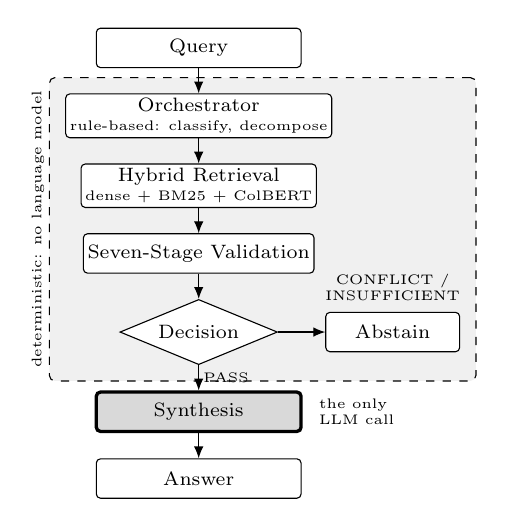
\begin{tikzpicture}[node distance=3.2mm and 6mm]
  \node[tbtbox, minimum width=26mm]                 (q)    {Query};
  \node[tbtbox, minimum width=26mm, below=of q]     (orch) {Orchestrator\\[-1pt]
        {\tiny rule-based: classify, decompose}};
  \node[tbtbox, minimum width=26mm, below=of orch]  (ret)  {Hybrid Retrieval\\[-1pt]
        {\tiny dense $+$ BM25 $+$ ColBERT}};
  \node[tbtbox, minimum width=26mm, below=of ret]   (val)  {Seven-Stage Validation};
  \node[tbtdec,  minimum width=20mm, below=of val]  (dec)  {Decision};
  \node[tbtbox, minimum width=17mm, right=6mm of dec] (abst) {Abstain};
  \node[tbtllm, minimum width=26mm, below=of dec]   (syn)  {Synthesis};
  \node[tbtbox, minimum width=26mm, below=of syn]   (ans)  {Answer};

  \draw[tbtarrow] (q)    -- (orch);
  \draw[tbtarrow] (orch) -- (ret);
  \draw[tbtarrow] (ret)  -- (val);
  \draw[tbtarrow] (val)  -- (dec);
  \draw[tbtarrow] (dec)  -- node[tbtlbl, right] {PASS} (syn);
  \draw[tbtarrow] (dec)  -- (abst);
  \draw[tbtarrow] (syn)  -- (ans);

  \node[tbtlbl, above=0.8mm of abst, align=center] {CONFLICT /\\INSUFFICIENT};
  \node[tbtlbl, right=1.5mm of syn, align=left]    {the only\\LLM call};

  \begin{scope}[on background layer]
    \node[fit=(orch)(ret)(val)(dec)(abst), draw, dashed, rounded corners=2pt,
          fill=detzonefill, inner sep=2mm] (detzone) {};
  \end{scope}
  \node[tbtlbl, rotate=90, anchor=south, align=center] at (detzone.west)
        {deterministic: no language model};
\end{tikzpicture}
\caption{Trust Before Text architecture. Everything in the shaded region is
deterministic and contains no language model; synthesis is the single LLM
call. Synthesis is reachable only on a PASS verdict, so a CONFLICT or
INSUFFICIENT verdict abstains before the language model is invoked.}
\label{fig:arch}
\end{figure}

\subsection{Deterministic Orchestrator}
\label{sec:orchestrator}
The orchestrator is the control plane and contains no language-model calls.
On receiving a query it executes a fixed sequence of stages:
preprocess, classify, optionally decompose, retrieve, validate, decide,
and, only if permitted, synthesize.

\textit{Preprocessing} normalizes the query by collapsing whitespace and
expanding common English contractions, so that surface variants of the
same question reduce to a single canonical form before retrieval.
\textit{Classification} is a rule-based function that labels the query as
\texttt{simple} or \texttt{complex} using lexical cues for multi-part
intent; no model is invoked. For a \texttt{complex} query,
\textit{decomposition} is likewise rule-based: it splits the question into
ordered atomic sub-queries using conjunction and comparison patterns,
subject to a minimum sub-query length, rather than an LLM query expander.
This keeps decomposition reproducible and inspectable.

A \textit{retrieval dispatcher} issues each sub-query to the retrieval
module and aggregates the returned evidence. A \textit{validation
controller} passes the aggregated chunks to the validation pipeline and
receives a structured verdict. The \textit{decision engine} interprets
that verdict deterministically: a PASS routes the evidence to a
\textit{generation gatekeeper} that builds the evidence pack for the
language model, whereas a CONFLICT or INSUFFICIENT verdict routes to the
abstention path described in Section~\ref{sec:abstention}. Because each
transition is a pure function of its inputs, the route a query takes is
fully determined by the query and the corpus.

\subsection{Hybrid Retrieval}
\label{sec:retrieval}
Retrieval is tuned for recall, on the principle that judging trust is the
validation pipeline's responsibility, not the retriever's. The module runs
three complementary signals over a Qdrant~\cite{qdrant} index. Approximate
nearest-neighbor indexing over persistent storage of this kind is a
well-documented engineering bottleneck across the vector-database
space~\cite{jing2024vdbmssurvey}, including in production similarity-search
libraries such as Faiss~\cite{douze2025faisslibrary}; we note this as context for
the infrastructure choice, not as a claim that Qdrant is uniquely suited to
it.

\textit{Dense retrieval} embeds the query and each chunk with the
\texttt{all-MiniLM-L6-v2} sentence encoder~\cite{reimers2019sbert} and
scores them by cosine similarity,
\begin{equation}
\mathrm{sim}(q,d) \;=\; \frac{E_q \cdot E_d}{\lVert E_q\rVert\,\lVert E_d\rVert},
\label{eq:cosine}
\end{equation}
where $E_q$ and $E_d$ are the query and chunk embeddings. \textit{Sparse
retrieval} uses a BM25~\cite{robertson2009bm25} lexical vector with Qdrant's
inverse-document-frequency modifier, capturing exact-term matches that dense
embeddings can miss.
The dense and sparse candidate lists are fused by Reciprocal Rank Fusion,
\begin{equation}
\mathrm{RRF}(d) \;=\; \sum_{r \in \{\text{dense},\,\text{sparse}\}}
\frac{1}{k + \mathrm{rank}_r(d)},
\label{eq:rrf}
\end{equation}
where $\mathrm{rank}_r(d)$ is the rank of chunk $d$ in list $r$ and $k$ is
a rank-smoothing constant. RRF combines the two rankings without requiring
their scores to be on a common scale.

The fused candidates are then reranked by a ColBERT late-interaction
cross-encoder~\cite{khattab2020colbert} (\texttt{answerai-colbert-small-v1})
using the MaxSim operator,
\begin{equation}
\mathrm{score}(q,d) \;=\; \sum_{i \in q}\; \max_{j \in d}\;
E_{q_i} \cdot E_{d_j},
\label{eq:maxsim}
\end{equation}
which sums, over each query token $i$, its best match against any chunk
token $j$. Late interaction gives finer-grained relevance than a single
pooled vector while remaining far cheaper than a full cross-encoder over
the corpus. Each returned chunk carries its dense, sparse, fused, and
ColBERT scores together with source metadata, so downstream stages and the
final audit trail can see exactly why a chunk was retrieved.

\subsection{Seven-Stage Validation Pipeline}
\label{sec:validation}
The validation pipeline is the factual gatekeeper. It applies seven
deterministic stages in sequence (Table~\ref{tab:validation}), and
Fig.~\ref{fig:validation} depicts the flow. Stages 1 through 3 clean and
scope the evidence; Stage 4 tests it for internal contradiction; Stage 5
tests whether enough of it survives to answer the query; Stages 6 and 7
structure the survivors and emit the verdict.

\begin{table}[htbp]
\caption{Seven-Stage Evidence Validation Pipeline}
\label{tab:validation}
\centering
\small
\begin{tabularx}{\columnwidth}{@{}>{\bfseries}c l X@{}}
\toprule
\# & Stage & Function \\
\midrule
1 & Normalization      & Standardize retrieved chunk text. \\
2 & Deduplication      & Remove near-identical chunks (cosine $\geq 0.90$). \\
3 & Relevance filter   & Drop chunks below a relevance floor; scope evidence to the query. \\
4 & Conflict detection & Flag cross-document contradiction via three prongs (Sec.~\ref{sec:conflict}). \\
5 & Sufficiency check  & Decide whether surviving evidence is adequate to answer. \\
6 & Evidence structuring & Rank validated chunks into an ordered evidence pack. \\
7 & Abstention decision & Emit PASS, CONFLICT, or INSUFFICIENT. \\
\bottomrule
\end{tabularx}
\end{table}

\begin{figure}[htbp]
\centering
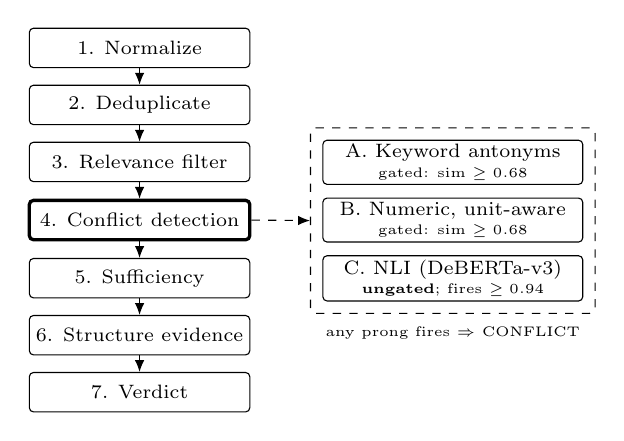
\begin{tikzpicture}[node distance=2.1mm and 8mm]
  \node[tbtbox, minimum width=28mm]                (s1) {1. Normalize};
  \node[tbtbox, minimum width=28mm, below=of s1]   (s2) {2. Deduplicate};
  \node[tbtbox, minimum width=28mm, below=of s2]   (s3) {3. Relevance filter};
  \node[tbtbox, minimum width=28mm, below=of s3, very thick]
                                                   (s4) {4. Conflict detection};
  \node[tbtbox, minimum width=28mm, below=of s4]   (s5) {5. Sufficiency};
  \node[tbtbox, minimum width=28mm, below=of s5]   (s6) {6. Structure evidence};
  \node[tbtbox, minimum width=28mm, below=of s6]   (s7) {7. Verdict};

  \draw[tbtarrow] (s1) -- (s2);
  \draw[tbtarrow] (s2) -- (s3);
  \draw[tbtarrow] (s3) -- (s4);
  \draw[tbtarrow] (s4) -- (s5);
  \draw[tbtarrow] (s5) -- (s6);
  \draw[tbtarrow] (s6) -- (s7);

  \node[tbtbox, minimum width=33mm, right=9mm of s4] (pB)
        {B. Numeric, unit-aware\\[-1pt]{\tiny gated: sim $\geq 0.68$}};
  \node[tbtbox, minimum width=33mm, above=1.6mm of pB] (pA)
        {A. Keyword antonyms\\[-1pt]{\tiny gated: sim $\geq 0.68$}};
  \node[tbtbox, minimum width=33mm, below=1.6mm of pB] (pC)
        {C. NLI (DeBERTa-v3)\\[-1pt]{\tiny \textbf{ungated}; fires $\geq 0.94$}};

  \begin{scope}[on background layer]
    \node[fit=(pA)(pB)(pC), draw, dashed, rounded corners=2pt,
          inner sep=1.5mm] (prongs) {};
  \end{scope}
  \draw[tbtarrow, dashed] (s4.east) -- (prongs.west);
  \node[tbtlbl, below=1mm of prongs, align=center]
        {any prong fires $\Rightarrow$ CONFLICT};
\end{tikzpicture}
\caption{The seven-stage validation pipeline, with Stage~4 expanded into
its three contradiction-detection prongs. The lexical and numeric prongs are
gated on lexical similarity; the NLI prong deliberately is not.}
\label{fig:validation}
\end{figure}

\subsubsection{Cross-Document Conflict Detection}
\label{sec:conflict}
Stage~4 is the pipeline's most distinctive component and the one most
responsible for catching disagreements that retrieval alone would blend
together. For each cross-document pair of chunks, it first restricts each
chunk to the sentences that mention the query's content terms, so that a
contradiction in a passage unrelated to the question cannot trigger a false
abstention. It then applies three prongs, illustrated in
Fig.~\ref{fig:conflict}.

\begin{figure}[htbp]
\centering
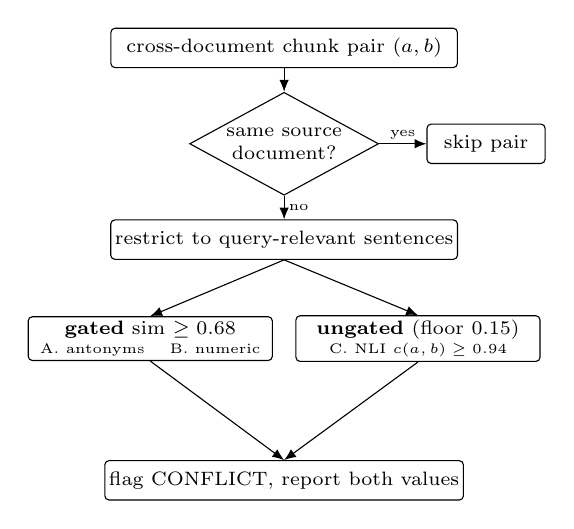
\begin{tikzpicture}
  \node[tbtbox, minimum width=44mm]                        (pair)
        {cross-document chunk pair $(a,b)$};
  \node[tbtdec, minimum width=24mm, below=3mm of pair]     (same)
        {same source\\document?};
  \node[tbtbox, minimum width=15mm, right=6mm of same]     (skip) {skip pair};
  \node[tbtbox, minimum width=44mm, below=3mm of same]     (scope)
        {restrict to query-relevant sentences};

  \node[tbtbox, minimum width=31mm] (gate) at ([xshift=-17mm, yshift=-10mm]scope.south)
        {\textbf{gated} sim $\geq 0.68$\\[-1pt]
         {\tiny A. antonyms \quad B. numeric}};
  \node[tbtbox, minimum width=31mm] (ung)  at ([xshift=17mm, yshift=-10mm]scope.south)
        {\textbf{ungated} (floor 0.15)\\[-1pt]
         {\tiny C. NLI $c(a,b) \geq 0.94$}};

  \node[tbtbox, minimum width=44mm] (flag) at ([yshift=-28mm]scope.south)
        {flag CONFLICT, report both values};

  \draw[tbtarrow] (pair)  -- (same);
  \draw[tbtarrow] (same)  -- node[tbtlbl, above] {yes} (skip);
  \draw[tbtarrow] (same)  -- node[tbtlbl, right] {no}  (scope);
  \draw[tbtarrow] (scope.south) -- (gate.north);
  \draw[tbtarrow] (scope.south) -- (ung.north);
  \draw[tbtarrow] (gate.south)  -- (flag.north);
  \draw[tbtarrow] (ung.south)   -- (flag.north);
\end{tikzpicture}
\caption{Conflict-detection decision flow. The cheap lexical and numeric
prongs are gated on high lexical similarity; the NLI prong is ungated on
similarity and fires only at a high contradiction score. This asymmetry is
deliberate: semantic contradictions often share little surface vocabulary.}
\label{fig:conflict}
\end{figure}

\textbf{Prong A, keyword antonyms.} A curated antonym and negation check
fires when two spans express opposing terms (for example
\textit{permitted} versus \textit{prohibited}). Because this prong is cheap
and precise, it is gated on high lexical similarity,
$\mathrm{sim}(a,b) \geq \tau_{\text{lex}}$ with $\tau_{\text{lex}} = 0.68$,
so that it only compares spans that are actually discussing the same thing.

\textbf{Prong B, unit-aware numeric.} This prong flags two spans that state
different values for the same quantity (for example a probationary period
of three months versus six months). It is unit-context aware, comparing
numbers only when they refer to the same attribute, and, like Prong~A, it
is gated on $\mathrm{sim}(a,b) \geq \tau_{\text{lex}}$.

\textbf{Prong C, natural language inference.} Pairing dense retrieval with an
NLI-trained verification step follows prior evidence-retrieval systems for
fact-checking, where NLI-trained dense retrievers were shown to outperform
sparse baselines at surfacing the passages that actually support or
contradict a claim~\cite{samarinas2020latent}; we reuse that pairing for
contradiction rather than support. A DeBERTa-v3~\cite{he2021deberta}
NLI cross-encoder (\texttt{cross-encoder/nli-deberta-v3-base}) scores each
span pair for contradiction in both directions,
\begin{equation}
c(a,b) \;=\; \max\bigl(\mathrm{contra}(a,b),\,\mathrm{contra}(b,a)\bigr),
\label{eq:nli}
\end{equation}
and a conflict is flagged when $c(a,b) \geq \tau_{\text{nli}}$ with
$\tau_{\text{nli}} = 0.94$. Unlike the lexical and numeric prongs, this
prong is \textbf{not} gated on lexical similarity; only a small floor
($0.15$) is applied to avoid spending NLI computation on clearly unrelated
spans. This asymmetry is deliberate: semantic contradictions frequently
share little surface vocabulary, so gating NLI on lexical similarity would
silently suppress exactly the conflicts it exists to catch. A pair is
declared conflicting if any prong fires:
\begin{equation}
\mathrm{conflict}(a,b) \;=\;
\mathrm{A}(a,b)\;\vee\;\mathrm{B}(a,b)\;\vee\;\mathrm{C}(a,b).
\label{eq:conflict}
\end{equation}

\subsubsection{Sufficiency}
\label{sec:sufficiency}
Stage~5 imposes three hard requirements and a quality requirement
satisfied by either of two signals. Writing $n$ for the count of
relevant chunks, $\bar{s}$ for their average calibrated score,
$\mathrm{cov}$ for the fraction of the query's content words present
in the evidence, and $\mathrm{pres}$ for the fraction of the query's
focus terms that appear anywhere in the evidence,
\begin{equation}
\begin{split}
\mathrm{sufficient} \;\Longleftrightarrow\;\;
& (n \geq 1)\,\wedge\,(\exists\,\text{relevant chunk})\\[2pt]
& \wedge\;(\mathrm{pres} \geq \tau_{\text{focus}})\\[2pt]
& \wedge\;\bigl(\bar{s} \geq 0.65 \,\vee\, \mathrm{cov} \geq 0.55\bigr).
\end{split}
\label{eq:suff}
\end{equation}
The third requirement ($\mathrm{pres} \geq \tau_{\text{focus}}$,
default $\tau_{\text{focus}} = 0.5$) is a hard presence test, not a
threshold on a score: a majority of the query's rarest content words
must appear in the evidence at all. This is what refuses a question the
corpus genuinely does not cover — two gap queries (Corpus~1 Q051,
Corpus~2 Q017) were passing H2/H4 through marginal score or coverage
while their subject was absent from the corpus entirely. The cost of
this fix is three answerable queries that now over-abstain because the
corpus answers them in different vocabulary than the query used;
an exhaustive search over 2{,}304 focus configurations found no setting
that closes both gap leaks and passes all three paraphrase misses,
for reasons documented in Section~\ref{sec:limitations}.


\subsection{Synthesis and Faithfulness Verification}
\label{sec:synthesis}
On a PASS verdict, the generation gatekeeper builds a structured evidence
pack from the validated chunks and passes it, and only it, to a
Groq-hosted Llama-3 model, which is instructed to answer with inline
citation markers referencing specific chunks. The model has no access to
unvalidated content.

After generation, the system runs a post-generation \textbf{NLI
faithfulness check}. Reusing the same DeBERTa-v3 NLI model, it splits the
answer into sentences and, for each sentence, tests whether any evidence
chunk entails it; the faithfulness score is the fraction of answer
sentences so supported. If this score falls below a threshold of $0.70$,
the answer is returned with a visible caution prefix that reports how many
sentences lacked entailment. This is a transparency signal rather than a
hard gate: it surfaces weakly supported generation to the reader instead of
silently suppressing it. The returned object carries the citations, the
faithfulness score, and the list of any unsupported sentences, so the
output is inspectable rather than opaque.

\subsection{Structural Abstention}
\label{sec:abstention}
Abstention is a property of the pipeline, not a behavior of the model. The
orchestrator cannot reach synthesis without a PASS verdict, so when
validation reports CONFLICT or INSUFFICIENT the language model is never
called. The abstention response is auditable: it names the failing stage
and, for a conflict, the two clashing documents together with the specific
values that disagree. A representative conflict abstention reads:
\begin{quote}\small\itshape
``Cannot synthesize an answer: the evidence contains contradictory
information (probationary period: 3 months in the Employee Handbook vs.\
6 months in Recruitment \& Onboarding).''
\end{quote}
This is the operational difference from systems whose safety rests on a
learned or prompted tendency: here, a query that fails verification has no
path to a generated answer.

% ─────────────────────────────────────────────────────────────────────────────
\section{Implementation}
\label{sec:impl}

The system is implemented in Python~3.10 as a set of single-responsibility
modules that communicate through fixed, typed schemas. This section
documents the technology stack, the inter-module contracts, the complete
set of deterministic thresholds, and the steps taken for reproducibility.

\subsection{Technology Stack}
The retrieval index is a local, persistent Qdrant collection holding three
vectors per chunk: a dense \texttt{all-MiniLM-L6-v2} embedding (384
dimensions), a BM25 sparse vector with Qdrant's inverse-document-frequency
modifier, and ColBERT token-level multivectors from
\texttt{answerai-colbert-small-v1}. Contradiction and faithfulness checks
share a single \texttt{cross-encoder/nli-deberta-v3-base} model instance.
Synthesis is performed by a Groq-hosted Llama-3 model behind an interface
that abstracts the backend, so alternative providers can be substituted
without touching the pipeline. A FastAPI service exposes document-upload
and query endpoints and static-mounts a lightweight HTML, CSS, and
JavaScript frontend. Table~\ref{tab:stack} summarizes the stack.

\begin{table}[htbp]
\caption{Core Technology Stack}
\label{tab:stack}
\centering
\small
\begin{tabularx}{\columnwidth}{@{}l X@{}}
\toprule
Component & Technology \\
\midrule
Language          & Python 3.11 \\
Vector database   & Qdrant (local persistent) \\
Dense embedding   & \texttt{all-MiniLM-L6-v2} (384-d) \\
Sparse retrieval  & BM25 with Qdrant IDF modifier \\
Reranker          & ColBERT \texttt{answerai-colbert-small-v1} \\
NLI model         & \texttt{cross-encoder/nli-deberta-v3-base} \\
Synthesis LLM     & Groq-hosted Llama-3 (pluggable backend) \\
Service / UI      & FastAPI backend, static HTML/CSS/JS frontend \\
\bottomrule
\end{tabularx}
\end{table}

\subsection{Inter-Module Contracts}
Modules never pass free-form text between stages. Each stage returns a
typed object with a fixed schema, which makes the pipeline unit-testable
with mocked inputs and lets any single component be swapped in isolation.
The validation pipeline returns a verdict object carrying the ranked
evidence, the two decision flags, a confidence score, the count of
relevant chunks, and, on failure, a named abstention reason. Synthesis
returns an object carrying the answer, its citations, the faithfulness
score, and any sentences that failed the entailment check. Because the
decision flags and the abstention reason are explicit fields rather than
parsed from prose, the orchestrator's branching is a direct function of the
schema, not an interpretation of generated text.

\subsection{Deterministic Thresholds}
Every gate in the pipeline is a named constant, listed in full in
Table~\ref{tab:thresholds}. This matters for two reasons. First, it makes
the system's behavior fully specified: given the corpus and these
constants, the verdict for any query is determined. Second, it separates
the two kinds of parameter this paper is careful to distinguish. Most
thresholds are fixed structural defaults that encode design decisions, such
as the deduplication cutoff or the similarity gate on the cheap conflict
prongs. Three are calibrated to Corpus 1, the primary evaluation corpus
described in Section~\ref{sec:eval}: the NLI contradiction threshold
($0.94$) and the two sufficiency signals (average score $0.65$, query
coverage $0.55$). Three more were selected later, using both corpora: the
query-span floor ($0.35$), the focus-presence fraction ($0.50$), which
closed two gap leaks, and the answerhood margin ($5.5$). Of the 20 active
decision constants (Appendix~\ref{app:constants}), the other 14 are
structural. These same values are used, unmodified, on every corpus in
this paper, including the second corpus introduced in
Section~\ref{sec:corpus2} as a generalization test; no threshold is
re-fitted per corpus. The calibrated thresholds are the ones
Section~\ref{sec:limitations} flags as requiring re-fitting on a new
corpus; the transferable contribution is the method for placing them, not
the specific values.

\begin{table}[htbp]
\caption{Deterministic Thresholds. The first three calibrated values are
fitted on Corpus 1 only; the query-intent gate, focus presence and the
answerhood margin were selected using both corpora. Appendix~\ref{app:constants}
lists all 20 active decision constants. Structural values are
fixed design defaults and apply unchanged to every corpus.}
\label{tab:thresholds}
\centering
\small
\begin{tabularx}{\columnwidth}{@{}X c c l@{}}
\toprule
Threshold & Value & Stage & Type \\
\midrule
Duplicate similarity     & 0.90 & 2 & Structural \\
Relevance ratio          & 0.30 & 3 & Structural \\
Min relevance score      & 0.05 & 3 & Structural \\
Min chunk score          & 0.60 & 3 & Structural \\
Conflict similarity gate & 0.68 & 4 & Structural \\
NLI similarity floor     & 0.15 & 4 & Structural \\
NLI contradiction        & 0.94 & 4 & \textbf{Calibrated} \\
Min chunks               & 1    & 5 & Structural \\
Min average score        & 0.65 & 5 & \textbf{Calibrated} \\
Min query coverage       & 0.55 & 5 & \textbf{Calibrated} \\
Prefetch limit           & 20   & Ret. & Structural \\
Faithfulness             & 0.70 & Syn. & Structural \\
Query-intent gate        & 0.35 & 4 & \textbf{Calibrated} \\
Anchor: require both     & yes  & 4 & Structural \\
Min chunks for avg suff. & 2    & 5 & Structural \\
Min focus presence       & 0.50 & 5 & \textbf{Calibrated} \\
Answerhood margin        & 5.5  & 4 & \textbf{Calibrated} \\

\bottomrule
\end{tabularx}
\end{table}

\subsection{Reproducibility}
Three provisions make the evaluation reproducible. The dataset is released
in full: the 11-document corpus, the 78 queries with gold labels, and the
ground-truth fact map of 45 facts, 4 planted conflicts, and 6 deliberate
gaps. Every calibrated threshold is overridable through an environment
variable with the documented default, so the calibration sweep can be
reproduced without editing code. Finally, the index records a manifest of
the exact embedding, sparse, and reranker model names used to build it, and
the service rebuilds the collection automatically if any of those models
changes, preventing a silent mismatch between stored vectors and the models
querying them.

One value set (Appendix~\ref{app:constants}) is used for every post-fix
result and the external benchmark. The decision layer contains no sampling
and needs no seed, and the accuracy runs make no LLM calls. Every LLM call
uses temperature 0 except the baseline consistency check (5 unseeded reruns
at temperature 0.7); the invariance transforms use seed 20260819. The
post-merge runs used Python 3.11.9; dependencies are given as lower bounds,
not pinned versions.

\subsection{Interactive Interface}
Beyond the batch evaluation harness, the system runs as an interactive
service. A user uploads policy documents and submits queries through the
frontend, and each answer is displayed alongside its verified inline
citations, its confidence score, and its faithfulness score, so that the
evidence behind an answer, or the reason for an abstention, is visible at
the point of use.

% ─────────────────────────────────────────────────────────────────────────────
\section{Evaluation}
\label{sec:eval}

\subsection{Dataset and Setup}
Evaluation uses two corpora. The primary corpus, referred to as
\textbf{Corpus 1} throughout, is an authored collection of 11 enterprise HR
policy documents for a fictional company, Meridian Grid Technologies; it is
the corpus every threshold in this paper was calibrated on, and it is the
subject of every table and figure in this section unless a table is
explicitly marked otherwise. A second, independently authored corpus in a
different domain, Corpus 2, is introduced in
Section~\ref{sec:corpus2} as a held-out generalization test and was never
used to fit any threshold of the frozen system (the later fixes of
Section~\ref{sec:post_eval_fixes} were selected using both corpora, so
post-fix Corpus~2 numbers are in-sample). The documents contain real
numbered clauses under standard headings and cross-reference one another, as
genuine policy sets do. The corpus was authored to a fixed fact map first,
so that every query's gold label is known by construction rather than
assigned after the fact. This is a controlled-evaluation strength and, at
the same time, an honest limitation: the corpus is single-domain and
single-company, and we do not claim generalization from it. The ground
truth comprises 45 facts, 4 planted cross-document conflicts, and 6
deliberate gaps. From this we derive 78 queries, spanning seven phrasing
types (single-fact, multi-part, cross-document comparison, conflict-probing,
out-of-scope, aggregation, and applied-scenario), partitioned into 46
answerable, 16 conflict, and 16 insufficient queries. All 78 were
text-verified against the documents. Unless stated otherwise, the results in
Sections~\ref{sec:eval} through~\ref{sec:corpus2} are for the frozen system;
Section~\ref{sec:post_eval_fixes} reports the system after the later fixes.

\subsection{Metrics}
We report decision-level metrics, because the system's contribution is the
decision to answer, flag a conflict, or abstain. For the conflict class we
report precision, recall, and their harmonic mean,
\begin{equation}
P = \frac{TP}{TP+FP}, \quad
R = \frac{TP}{TP+FN}, \quad
F_1 = \frac{2PR}{P+R}.
\label{eq:prf}
\end{equation}
Overall decision accuracy is the fraction of the 78 queries assigned the
correct one of the three labels. The safety-critical metric is the
\textit{unsafe-answer rate}: of the 32 queries that must not be answered
(16 conflict, 16 insufficient), the fraction the system nonetheless
answered. Finally, to make the determinism claim measurable rather than
asserted, we define \textit{decision consistency} as the fraction of
queries whose decision is invariant across repeated runs,
\begin{equation}
\mathrm{consistency} = \frac{1}{|Q|}\sum_{q \in Q}
\mathbbm{1}\!\left[\,\forall\,i,j:\; d_i(q) = d_j(q)\,\right],
\label{eq:consistency}
\end{equation}
where $d_i(q)$ is the decision on query $q$ in run $i$. For Trust Before
Text this equals $1.0$ by construction, since the decision path contains no
stochastic component; the corresponding measurement for a prompted model is
reported in Section~\ref{sec:baseline}.

\subsection{Summary: Both Corpora, Both Systems}
\label{sec:summary_table}
Before the detailed results, Table~\ref{tab:summary} places every
by-construction guarantee this paper claims side by side, on both corpora
and against the prompted baseline. We state the tradeoff plainly rather
than hide it: accuracy is the one row where our system is not the strongest
number, and on Corpus 2 it falls well below the prompted baseline. What we
report instead is that every other row, determinism, injection immunity,
and (with the caveat in Table~\ref{tab:heldvsdrifted}) attribution, holds
regardless of that accuracy drop, because those properties come from the
architecture rather than from the model's average-case performance. A lower
accuracy number is the cost of the guarantee, not evidence against it, and
Table~\ref{tab:summary} is where that exchange is easiest to see at a
glance. The two decision-layer injection cells for the baseline are marked
not applicable because a prompted model has no separate decision layer to
test in isolation: the model itself is the decision, so the fixed-injection
study (Section~\ref{sec:adv-injection}) instead measures its overall attack
success rate, and no baseline injection test was run on Corpus 2 at all,
consistent with Section~\ref{sec:corpus2}'s spot-check being decision-layer
only.

\begin{table}[htbp]
\caption{Guarantee Properties Across Both Corpora and Both Systems (Frozen System). Accuracy
drifts with the corpus; every other row holds by construction wherever it
applies.}
\label{tab:summary}
\centering
\scriptsize
\setlength{\tabcolsep}{3pt}
\begin{tabular}{@{}>{\raggedright\arraybackslash}p{0.28\columnwidth}
                    *{4}{>{\centering\arraybackslash}p{0.145\columnwidth}}@{}}
\toprule
\multirow{2}{*}{Metric} & \multicolumn{2}{c}{Corpus 1} & \multicolumn{2}{c}{Corpus 2} \\
 & ours & base. & ours & base. \\
\midrule
Decision accuracy                       & 92.3\%        & 97.4\% & 66.7\% & 98.7\% \\
Conflict recall                         & 100\%         & 93.8\% & 100\%           & 93.8\% \\
Unsafe answers\textsuperscript{a}       & \textbf{0}    & 1      & 4      & 1 \\
Decision flips                          & \textbf{0\%}\textsuperscript{b}  & 1.3\%\textsuperscript{c}  & \textbf{0\%}\textsuperscript{b}    & 1.3\%\textsuperscript{c} \\
Injection obeyed\textsuperscript{d}     & \textbf{0/45} & n/a    & \textbf{0/15}\textsuperscript{e} & n/a \\
\bottomrule
\end{tabular}

\vspace{3pt}
\raggedright\scriptsize
\textsuperscript{a}Of 32 conflict-or-gap queries that must not be answered.
\textsuperscript{b}Ours: determinism by construction, since the decision
path has no stochastic component and no temperature parameter; verified by
an 8-query replay, not a repeated-sampling protocol.
\textsuperscript{c}Baseline: across 5 repeated runs at temperature 0.7.
\textsuperscript{d}Decision layer only; a prompted baseline has no separate
decision layer to isolate, so its overall attack success rate is reported
instead in Section~\ref{sec:adv-injection}.
\textsuperscript{e}15-case Corpus 2 spot-check (Section~\ref{sec:corpus2}),
not a repeat of the full 45-case Corpus 1 study.
\end{table}

\subsection{Main Results}
Table~\ref{tab:results} reports the primary results. The system reaches
92.3\% decision accuracy (72 of 78). Conflict recall is perfect (16 of 16),
conflict precision is 0.727 (16 of 22), giving a conflict $F_1$ of 0.842.
Answer recall is 87.0\% (40 of 46) and gap recall is 100\% (16 of 16). The
headline safety result is that the unsafe-answer rate is exactly zero:
across all 32 queries that should trigger abstention, the system answered
none.

\begin{table}[htbp]
\caption{Main Results on Corpus 1 (78 Queries)}
\label{tab:results}
\centering
\small
\begin{tabularx}{\columnwidth}{@{}X r@{}}
\toprule
Metric & Value \\
\midrule
Decision accuracy         & 92.3\% (72/78) \\
Conflict recall           & 1.000 (16/16) \\
Conflict precision        & 0.727 (16/22) \\
Conflict $F_1$            & 0.842 \\
Answer recall             & 87.0\% (40/46) \\
Gap / insufficient recall & 100\% (16/16) \\
\textbf{Unsafe answers}   & \textbf{0 / 32 (0\%)} \\
\bottomrule
\end{tabularx}
\end{table}

The confusion matrix in Table~\ref{tab:confusion}, plotted as a heatmap in
Figure~\ref{fig:confusion_heat}, shows why this matters.
Every off-diagonal cell is zero except one: six answerable queries were
flagged as conflicts. No conflict was missed, no gap was answered, and no
query was answered when it should have abstained. In other words, every one
of the system's six errors is an over-cautious abstention, not a piece of
misinformation. This asymmetry, errors that only ever cost a refusal and
never produce a false answer, is the practical meaning of the safety
guarantee.

\begin{table}[htbp]
\caption{Confusion Matrix, Corpus 1 (rows: gold label, columns: system decision)}
\label{tab:confusion}
\centering
\small
\begin{tabularx}{\columnwidth}{@{}l *{3}{c} c@{}}
\toprule
Gold $\downarrow$ / Decision $\rightarrow$ & Answer & Conflict & Insuff. & Total \\
\midrule
Answer        & 40 & 6  & 0  & 46 \\
Conflict      & 0  & 16 & 0  & 16 \\
Insufficient  & 0  & 0  & 16 & 16 \\
\bottomrule
\end{tabularx}
\end{table}

\begin{figure}[htbp]
\centering
\IfFileExists{fig4_confusion_matrix.pdf}
  {\includegraphics[width=0.85\columnwidth]{fig4_confusion_matrix.pdf}}
  {\figplaceholder{3x3 confusion-matrix heatmap: only off-diagonal cell is
   Answer$\to$Conflict = 6.}}
\caption{Confusion-matrix heatmap, Corpus 1. The only non-zero off-diagonal
cell is the six answerable queries flagged as conflicts.}
\label{fig:confusion_heat}
\end{figure}

\subsection{Ablation}
Table~\ref{tab:ablation} isolates the effect of the two decisive design
choices, measured on the full 78-query corpus. A validation-enabled
baseline configuration scores 67.9\%. Replacing the conjunctive sufficiency
rule with the disjunction of Equation~\eqref{eq:suff}, so that a query
passes on either a high average score or high coverage, raises accuracy to
83.3\%. Calibrating the NLI contradiction threshold to 0.94 and removing an
over-eager comparison override, which together suppress false conflicts
while recovering genuine comparison conflicts, brings the system to 92.3\%.
The gains are cumulative and each corresponds to a specific, inspectable
change, shown as a running total in Figure~\ref{fig:ablation}.

\begin{table}[htbp]
\caption{Ablation on Corpus 1 (78 Queries)}
\label{tab:ablation}
\centering
\small
\begin{tabularx}{\columnwidth}{@{}X r@{}}
\toprule
Configuration & Accuracy \\
\midrule
Validation baseline                          & 67.9\% (53/78) \\
\quad + Sufficiency AND$\rightarrow$OR       & 83.3\% (65/78) \\
\quad + NLI 0.94 and remove comparison override & 92.3\% (72/78) \\
\bottomrule
\end{tabularx}
\end{table}

\begin{figure}[htbp]
\centering
\IfFileExists{fig5_ablation.pdf}
  {\includegraphics[width=\columnwidth]{fig5_ablation.pdf}}
  {\figplaceholder{Ablation bar chart: 67.9\% $\to$ 83.3\% $\to$ 92.3\%.}}
\caption{Cumulative ablation on Corpus 1: each architectural change and its
effect on decision accuracy.}
\label{fig:ablation}
\end{figure}

\subsection{NLI Score Separation}
Figure~\ref{fig:nli} plots the NLI contradiction scores of the true planted
conflicts against those of the false conflicts, with the 0.94 threshold
drawn between them. The true conflicts cluster tightly at the top (0.965 and
above), and most false conflicts fall well below the threshold. The figure
also makes the residual limitation visible: two false conflicts score above
every true conflict (0.9996 and 0.9998), so no choice of threshold can
remove them without also discarding real conflicts. This is the empirical
basis for the core open problem discussed in Section~\ref{sec:limitations}.

\begin{figure}[htbp]
\centering
\IfFileExists{fig6_nli_separation.pdf}
  {\includegraphics[width=\columnwidth]{fig6_nli_separation.pdf}}
  {\figplaceholder{NLI score separation: true conflicts $\geq 0.965$ vs
   false $\leq 0.92$, threshold line at 0.94; two false outliers above all
   true conflicts.}}
\caption{NLI contradiction scores for true versus false conflicts, Corpus 1.
The threshold at 0.94 sits in the gap between the two populations, except
for two false conflicts that score above every true conflict.}
\label{fig:nli}
\end{figure}

\subsection{Prompted-LLM Baseline}
\label{sec:baseline}
To test whether the architectural guarantee buys anything a well-prompted
model does not already provide, we evaluate a strong prompted baseline on
the identical 78 queries. The baseline is a Groq-hosted
\texttt{llama-3.3-70b-versatile} model given the same retrieved evidence our
pipeline produces, capped at the top 12 passages per query with each
passage labelled by its source document. The system prompt instructs the
model to answer only from the passages, to reply \texttt{INSUFFICIENT} when
the answer is absent, and to reply \texttt{CONFLICT} with both values and
their source documents when two passages disagree. Each query is run once at
temperature 0 for the accuracy, attribution, and leakage measurements, and
five additional times at temperature 0.7 for the determinism test.

The baseline is a genuinely strong competitor, and we report that plainly.
It reaches 97.4\% decision accuracy (76 of 78), higher than our 92.3\%. Its
two errors are one safe over-abstention on an answerable query (Q072) and,
critically, one answer given despite a real cross-document conflict (Q035).
Its confusion matrix is shown in Table~\ref{tab:baseline_confusion}.

\begin{table}[htbp]
\caption{Baseline Confusion Matrix, Corpus 1 (rows: gold, columns: baseline decision)}
\label{tab:baseline_confusion}
\centering
\small
\begin{tabularx}{\columnwidth}{@{}l *{3}{c} c@{}}
\toprule
Gold $\downarrow$ / Baseline $\rightarrow$ & Answer & Conflict & Insuff. & Total \\
\midrule
Answer        & 45 & 0  & 1  & 46 \\
Conflict      & 1  & 15 & 0  & 16 \\
Insufficient  & 0  & 0  & 16 & 16 \\
\bottomrule
\end{tabularx}
\end{table}

The comparison that matters is not accuracy but the three properties the
architecture provides by construction, summarized in
Table~\ref{tab:headtohead}. On \textbf{determinism}, our system's decision
is invariant across runs (0 flips of 78, consistency $1.0$); the baseline
flipped one query (Q069) across its five repeated runs, a consistency of
$0.987$. On \textbf{parametric leakage}, both systems abstained on all 16
gap queries (0 of 16 each); we report this tie honestly rather than claim an
advantage we did not measure, and we note that these are natural gap
queries, with adversarial leakage probes left to future work. On
\textbf{attribution quality}, our system named both clashing documents and
both values on all 16 conflicts (16 of 16 full marks); the baseline earned
full marks on 14 of 16 (mean $2.875$ of 3), missing the two points on the
conflict it failed to flag. On the direct \textbf{safety} measure, our
unsafe-answer rate is 0 of 32 by construction, while the baseline's is 1 of
32 (Q035).

\begin{table}[htbp]
\caption{Trust Before Text versus a Prompted-LLM Baseline, Corpus 1. The
baseline is more accurate; our system holds the reliability properties it
lacks.}
\label{tab:headtohead}
\centering
\small
\begin{tabularx}{\columnwidth}{@{}X c c@{}}
\toprule
Property & Trust Before Text & Prompted baseline \\
\midrule
Decision accuracy              & 92.3\% (72/78)      & 97.4\% (76/78) \\
Decision consistency (5 runs)  & \textbf{1.000 (0 flips)} & 0.987 (1 flip) \\
Parametric leakage (16 gaps)   & 0/16                & 0/16 \\
Conflict attribution (3/3)     & \textbf{16/16}      & 14/16 (2.875/3) \\
Unsafe answers                 & \textbf{0/32}       & 1/32 (Q035) \\
\bottomrule
\end{tabularx}
\end{table}

The result is exactly the intended one. A well-prompted model can be more
accurate on average, yet it remains a probabilistic system: it can change
its decision from one run to the next, and on this corpus it produced one
confidently wrong answer to a question the documents genuinely contradict.
Trust Before Text cannot, because the model is never reached on a conflict.
Higher average accuracy and a worst-case safety guarantee are different
things, and the baseline demonstrates the first while lacking the second.

\subsection{Generalization: A Second Corpus}
\label{sec:corpus2}
Every threshold in Table~\ref{tab:thresholds} was calibrated on Corpus 1
alone (Section~\ref{sec:impl}). To test whether that calibration, and the
architecture's guarantees more broadly, transfer to unseen content, we ran
the identical frozen system, with no threshold or decision logic changed,
on a second corpus authored independently to the same fixed-fact-map
methodology but in a deliberately different domain and convention: US
university academic regulations, against Corpus 1's UK enterprise HR
policies. Because Corpus 2 played no role in choosing any threshold of the frozen
system, this is a genuine held-out generalization test of that system rather
than a second round of tuning. It was held out only for this first run: the
later fixes of Section~\ref{sec:post_eval_fixes} used both corpora.
The second corpus matches Corpus 1's structure exactly
(11 documents including one superseded pair, 78 queries split 46 answer, 16
conflict, and 16 insufficient, with 4 planted conflicts and 6 gaps), so any
change in results is attributable to content, not test design.

The outcome separates cleanly into properties that transferred and numbers
that did not (Table~\ref{tab:corpus2}), and we report the accuracy side of
that split first because it is the part where our system does not win.
Decision accuracy fell from 92.3\% to
66.7\% (52 of 78), while the prompted baseline rose slightly to 98.7\%,
widening Corpus 1's near-tie into a clear accuracy gap. The drop is dominated
by conflict over-flagging: conflict F1 fell from 0.84 to 0.60, driven by
precision (0.43, from 16 true flags against 21 false ones) rather than by any
missed conflict. We report recall and precision jointly and lead with F1,
because recall staying at 16 of 16 is confounded with that precision collapse
and cannot be read as an independent success. Set against that drop,
determinism and structural attribution do not move at all between the two
corpora (Table~\ref{tab:heldvsdrifted}): the accuracy number is corpus-sensitive
precisely because it depends on the calibrated thresholds, while the
guarantees that do not depend on calibration are unaffected by the same
distribution shift that costs 26 points of accuracy. That is the tradeoff
this paper is built around, stated on the corpus where it is least
flattering to us.

The errors are mostly in the safe direction. Of 26 errors, 22 are conservative
(19 answerable queries flagged as conflicts, 2 gaps flagged as conflicts, and
1 answerable query abstained) and 4 are unsafe: gap queries answered instead
of abstained, so the unsafe-answer rate rose from 0 of 32 to 4 of 32 against
the baseline's 1 of 32. That gap leakage is a sufficiency-calibration effect,
distinct from the conflict issue, and is analyzed in
Section~\ref{sec:limitations}.

The precision collapse has a specific, nameable cause. Two documents, a
superseded course-registration policy and a general student handbook, each
sit inside a planted conflict and also share near-identical wording with
their usual partner on many unrelated facts. Seventeen of the nineteen false
conflicts involve one of these two documents, regardless of partner; twelve
of the nineteen are the exact conflicting pair itself (the superseded policy
against its replacement, or the handbook against the academic catalog).
Because these two documents are co-retrieved for almost any related query,
the query-unscoped conflict detector re-fires whenever they appear together,
correctly or not. This is Corpus 1's core open problem
(Section~\ref{sec:limitations}) amplified by document overlap, not a new
failure.

\begin{table}[htbp]
\caption{Corpus 2 (US academic regulations) against Corpus 1. By-construction
properties transfer; calibrated numbers drift.}
\label{tab:corpus2}
\centering
\small
\begin{tabularx}{\columnwidth}{@{}X c c c@{}}
\toprule
Metric & Corpus 1 (ours) & Corpus 2 (ours) & Corpus 2 (base.) \\
\midrule
Decision accuracy       & 92.3\% & 66.7\% & 98.7\% \\
Conflict $F_1$          & 0.84   & 0.60   & 0.97 \\
\quad precision         & 0.73   & 0.43            & 1.00 \\
\quad recall            & 1.00   & 1.00            & 0.94 \\
Unsafe answers (/32)    & 0      & 4      & 1 \\
\bottomrule
\end{tabularx}
\end{table}

\begin{table}[htbp]
\caption{What held versus what drifted across the two corpora.}
\label{tab:heldvsdrifted}
\centering
\small
\begin{tabularx}{\columnwidth}{@{}X l l@{}}
\toprule
Property & Type & Transfer \\
\midrule
Determinism (0 flips)          & by construction & held \\
Structural attribution (3/3)   & by construction & held \\
Conflict recall (16/16)        & empirical\textsuperscript{a} & entangled with precision \\
Decision accuracy              & calibrated      & drifted \\
Conflict precision             & calibrated      & drifted \\
Unsafe-answer rate             & calibrated      & drifted \\
\bottomrule
\end{tabularx}

\vspace{3pt}
\raggedright\scriptsize
\textsuperscript{a}Recall stayed at 16 of 16 on both corpora, but this is
not an independent by-construction guarantee: the same query-unscoped
firing that preserves recall is also what drives the precision collapse on
Corpus 2 (Table~\ref{tab:corpus2}).
\end{table}

\subsection{External Validation: RAMDocs}
\label{sec:ramdocs}
Both corpora in Sections~\ref{sec:eval} and~\ref{sec:corpus2} were authored by
this project to a fixed fact map, which is a controlled-evaluation strength
and, as Section~\ref{sec:limitations} states plainly, an open question about
generalization to content this project did not write and did not select
against. To address that question directly, we ran the current system,
the one in the ``current'' columns of Table~\ref{tab:fixes_headline}, against
RAMDocs~\cite{wang2025ramdocs}, an externally authored benchmark of 500
queries in which each query supplies several documents individually labeled
\texttt{correct}, \texttt{misinfo}, or \texttt{noise}. Neither the documents
nor the queries were seen during threshold calibration, and no threshold was
adjusted after this run; the grading rules were fixed in advance
(preregistration documented separately). A superseded earlier run exposed
gold labels in document names and was replaced by the run reported here, in
which every document is named only ``Document~$N$'' and no label or answer
field reaches any chunk or prompt. A prompted baseline (\texttt{gpt-oss-120b},
the model our synthesis uses here, temperature 0, instructed to answer only
from the passages and to reply \texttt{INSUFFICIENT} or \texttt{CONFLICT}
otherwise) ran on the same documents under the same names, and both systems
were graded by the same code on one protocol (Table~\ref{tab:ramdocs_main});
no baseline reply was empty. Because the first document is a correct one in
476 of the 500 records, both systems were also run with the documents in a
seeded random order; the results are given below.

\subsubsection{Task Correspondence and a Deliberate Deviation}
Table~\ref{tab:ramdocs_task} summarizes the correspondence. The one
methodological deviation from every other result in this paper is that
RAMDocs supplies its documents directly with each query, so retrieval is
bypassed: the documents are injected as already-retrieved evidence rather
than recovered from a Qdrant index. This means the RAMDocs result validates
the validation and decision layers on unseen content, but it does not
exercise Stage~3's relevance filtering the way live retrieval does (every
supplied document receives a uniform placeholder score above the relevance
floor), and it says nothing about whether our retrieval stage would have
surfaced the same documents unassisted. We report this as a scope
limitation on the result, not as a discovery made after the fact.

\begin{table}[htbp]
\caption{Task Correspondence, RAMDocs versus This System}
\label{tab:ramdocs_task}
\centering
\small
\begin{tabularx}{\columnwidth}{@{}l X X@{}}
\toprule
 & RAMDocs (published) & Trust Before Text (as run) \\
\midrule
Input & 1--12 labeled docs/query & Same docs, closed-book (retrieval bypassed) \\
Ambiguous queries & Multiple valid gold answers & Handled identically; no query-specific accommodation \\
LLM calls/query & 1 (baseline) to several (MADAM-RAG) & 1 (single synthesis call) \\
\bottomrule
\end{tabularx}
\end{table}

\subsubsection{Metric Non-Equivalence}
RAMDocs' own published table~\cite{wang2025ramdocs} scores every method,
including their best multi-round debate method, MADAM-RAG, by exact match
(EM): the output must contain every gold answer and no wrong one. We score
our system and the prompted baseline by EM, and we also report
\textit{safe rate}, the fraction of queries whose answer contains a gold
answer or that the system refused, because that is this paper's stated
thesis and EM has no abstention credit. \textbf{The published EM figures
come from different models, prompts, and no refusal option, so they are
context only, and nothing below is a claim that our system outscores
MADAM-RAG on their task.} Table~\ref{tab:ramdocs_main} reports what a
deterministic gate applied after a single LLM call does on data explicitly
designed to contain conflicting and misleading evidence, next to a prompted
baseline under the same protocol.

\begin{table}[htbp]
\caption{RAMDocs, 500 Queries, One Protocol. Ours and the prompted baseline
both use \texttt{gpt-oss-120b}, run on the same documents and graded by the
same code; Wilson 95\% intervals. Published EM scores are in
Table~\ref{tab:ramdocs_published}.}
\label{tab:ramdocs_main}
\centering
\footnotesize
\begin{tabularx}{\columnwidth}{@{}X r r@{}}
\toprule
Metric & Ours & Prompted baseline \\
\midrule
Refusal rate              & 31.4\% [27.5, 35.6] & 76.8\% [72.9, 80.3] \\
Exact match (EM)          & 18.0\% [14.9, 21.6] & 7.6\% [5.6, 10.3] \\
Misinformation asserted   & 2.8\% [1.7, 4.6]    & 1.0\% [0.4, 2.3] \\
Safe rate                 & 85.2\% [81.8, 88.0] & 94.8\% [92.5, 96.4] \\
Refusals justified        & 54.1\% (85/157)     & 54.4\% (209/384) \\
Answered: gold / misinfo  & 78.4\% / 4.1\% (of 343) & 77.6\% / 4.3\% (of 116) \\
\bottomrule
\end{tabularx}
\end{table}

\begin{table}[htbp]
\caption{Published exact-match scores on RAMDocs~\cite{wang2025ramdocs}
(Llama-3.3-70B unless noted; different prompts, no refusal option). Context
only: not the protocol of Table~\ref{tab:ramdocs_main}.}
\label{tab:ramdocs_published}
\centering
\small
\begin{tabularx}{\columnwidth}{@{}X r r@{}}
\toprule
Method & Calls/query & Score \\
\midrule
No RAG (Llama-3.3-70B)        & 1     & 5.8\% EM \\
Prompt-based RAG (Llama-3.3-70B) & 1  & 32.6\% EM \\
Self-reflection agent          & 2+    & 30.4\% EM \\
Speculative RAG                & 2+    & 30.6\% EM \\
Astute RAG                     & 2+    & 31.8\% EM \\
MADAM-RAG (Llama-3.3-70B)      & several & 34.4\% EM \\
MADAM-RAG (Qwen2.5-72B)        & several & 26.4\% EM \\
MADAM-RAG (GPT-4o-mini)        & several & 28.0\% EM \\
\bottomrule
\end{tabularx}
\end{table}

The prompted baseline is safer (94.8\% vs.\ 85.2\% safe rate, exact McNemar
$p<10^{-8}$) and asserts misinformation less often (1.0\% vs.\ 2.8\%,
exact McNemar $p=0.022$), largely by refusing 76.8\% of queries against our 31.4\%. Ours
answers far more correctly (EM 18.0\% vs.\ 7.6\%, $p<10^{-12}$) and is
comparable to the baseline per answered query (gold share $p=0.90$,
misinformation share $p=1.0$). Of the 343 queries ours answered, 60 (17\%)
match neither a gold nor a misinformation answer; the string-match grader
leaves them unscored, so they count as neither safe nor unsafe, and the
safe rate is a fraction of all 500 queries. The grader is lenient in one
direction: an answer containing both a gold and a wrong value counts as
safe. Counting any wrong value as unsafe gives 71.6\% safe for ours and
94.2\% for the baseline. With the documents shuffled, our gate makes the
identical decision on all 500 queries and the safe rate is 85.4\%
(misinformation asserted 4.0\%, EM 18.6\%); the baseline gives 93.6\%
(1.6\%, 8.0\%), so the comparison does not depend on document order.
Every baseline figure in this section comes from the recalculated run with
the prompt of Section~\ref{sec:baseline} (94.8\% safe in the original
order); an earlier run with a different baseline prompt is not reported,
because neither that prompt nor its per-query results are available.

Two observations temper any reading of Table~\ref{tab:ramdocs_published} as a
head-to-head win. First, the published numbers themselves show that extra
LLM calls buy almost nothing on this data: self-reflection, Speculative
RAG, and Astute RAG all score \textit{below} the single-call baseline, and
even MADAM-RAG's several-round debate reaches only 1.8 points above it.
This is evidence about what re-prompting an LLM to adjudicate conflicting
evidence does and does not fix, and it is the same argument this paper
makes about our own deterministic gate versus a prompted baseline in
Section~\ref{sec:baseline}, now corroborated on a benchmark we did not
author. Second, the prompted baseline in Table~\ref{tab:ramdocs_main} is a
prompt-only LLM, not our own retrieval and pipeline with the gate removed;
that same-metric, gate-removed ablation is scoped but not yet built, so
neither table isolates what the gate itself contributes.

\subsubsection{Abstention Quality on Unseen Data}
Of the 426 safe outcomes, 157 were abstentions and 269 were answers
containing a gold answer. Checked against RAMDocs' own per-document labels,
a check no comparator system's published number is scored against, only
54.1\% of those abstentions (85/157) coincided with a document actually
labeled \texttt{misinfo} (Table~\ref{tab:ramdocs_abstain}); the prompted
baseline's refusals line up at about the same rate (54.4\%, 209/384). The remaining
45.9\% abstained on queries that were merely ambiguous or noise-heavy rather
than contaminated. For scale, 243 of the 500 queries (48.6\%) contain a
misinformation document, so abstaining at random would line up about as
often: the observed 54.1\% (95\% interval 46.0\% to 62.1\%) is not
distinguishable from that (exact binomial test against 48.6\%,
$p=0.175$), and the abstention rate was 35.0\% on
queries with a misinformation document against 28.0\% on those without
($p=0.10$). We read this as a genuine limitation, not a hedge on the
headline number: on unseen content the system's abstentions track the
presence of misinformation only weakly.

\begin{table}[htbp]
\caption{RAMDocs Abstentions Checked Against Ground-Truth Document Labels}
\label{tab:ramdocs_abstain}
\centering
\small
\begin{tabularx}{\columnwidth}{@{}X r r@{}}
\toprule
 & Count & \% of abstentions \\
\midrule
Misinformation document present (justified)   & 85 & 54.1\% \\
No misinformation document present            & 72 & 45.9\% \\
\bottomrule
\end{tabularx}
\end{table}

\subsubsection{What This Result Does and Does Not Show}
RAMDocs closes one specific gap this paper is otherwise open about: it is
externally authored and was never used for design selection, so the result
is not subject to the self-authored-corpus concern that applies to Corpus~1
and Corpus~2 (Section~\ref{sec:limitations}). It does not close the others.
The run is closed-book, so it says nothing about retrieval; it was run in
two document orders (a superseded earlier run that exposed gold labels in
document names was discarded), which shows the gate's decisions do not
depend on order, but it is not a repeated-run consistency check of the
synthesised answers of the kind Table~\ref{tab:headtohead} runs for
Corpus~1; a prompted LLM is safer on it
(Table~\ref{tab:ramdocs_main}); and its safe-rate metric is not directly
comparable to the accuracy, $F_1$, and unsafe-answer figures reported
elsewhere in this paper. We treat it as one data point of external evidence
for the guarantee-versus-behavior claim, not as a replacement for the
held-out, same-domain test the paper still lacks.

\subsection{External Validation: MultiHop-RAG}
\label{sec:multihop}
A second externally authored benchmark, MultiHop-RAG (public release
\texttt{yixuantt/MultiHopRAG}), tests the full pipeline with retrieval, which
RAMDocs does not. The corpus is 609 news articles and 2{,}556 queries; we
indexed all 609 articles through the unchanged ingestion (22{,}131 chunks).
The comparison was preregistered before any query was run and is a new
measurement, not a repetition of an earlier sample. We drew 300 queries with a
fixed seed: 150 null queries (no answer in the corpus) and 50 each of
inference, comparison, and temporal queries, run in shuffled order. Our arm
makes no LLM call. The baseline is the prompted LLM of
Section~\ref{sec:baseline} (same E1 prompt, \texttt{gpt-oss-120b})
given the same retrieved passages. Because the provider's free tier rejected
requests above 8{,}000 tokens, the baseline receives at most 12 passages, a
cap fixed after a pilot and before the full run; our gate validates about 30.
Only 67.4\% of gold articles fall inside the baseline's 12 passages, so the
comparison is asymmetric, and we report it as such rather than correcting it.
Only decisions are graded, not answer content.

\begin{table}[htbp]
\caption{MultiHop-RAG, 300 Paired Queries (Wilson 95\% Intervals; Exact McNemar)}
\label{tab:multihop}
\centering
\small
\begin{tabularx}{\columnwidth}{@{}X r r r@{}}
\toprule
 & Ours & Baseline & $p$ \\
\midrule
Null queries answered (of 150)    & 56 (37.3\%) & 2 (1.3\%)   & $1.2\times10^{-14}$ \\
Answerable not answered (of 150)  & 78 (52.0\%) & 110 (73.3\%) & $5.8\times10^{-5}$ \\
Decision correct, strict (of 300) & 125 (41.7\%) & 188 (62.7\%) & $6.4\times10^{-7}$ \\
\bottomrule
\end{tabularx}
\end{table}

The result is mixed and we report all of it. The gate answers 56 of 150 null
queries against the baseline's 2 (95\% intervals 30.0\% to 45.3\% and 0.4\%
to 4.7\%), so on this benchmark it leaks answers into the gap far more often
than the prompted LLM. It also refuses fewer answerable queries (52.0\%
against 73.3\%), but 77 of its 78 refusals are conflict flags, not
insufficient-evidence abstentions, and the strict decision-correct rate is
significantly lower than the baseline's (41.7\% against 62.7\%, 95\% intervals
36.2\% to 47.3\% and 57.1\% to 67.9\%). Under a lenient grading in which any
abstention on a null query counts as correct, the difference is not
significant (55.3\% against 62.7\%, $p=0.055$; exploratory). One of the five
preregistered predictions failed: we predicted no significant difference in
strict correctness, and the baseline is significantly better.

Two mechanisms account for most of this, and both are failure patterns
already named in this paper. The gate tests relevance and coverage, not
whether the retrieved text contains the answer, so near-miss null queries
pass. Conflict detection flags disagreement between articles without
establishing that it concerns the question: 77 false conflicts on answerable
queries and 41 on null ones. Retrieval is not the cause. Across sub-queries
89.0\% of gold articles are retrieved, and article recall at rank five for the
original question is 59.6\%, the same pattern as the paragraph on retrieval
recall in Section~\ref{sec:retrieval_recall}. The baseline's refusals are not
explained by the cap alone: it refused 38 of 60 answerable queries even when
every gold article was sent, and 72 of 90 when some were cut (exploratory).

This benchmark therefore supports the paper's claim only in its structural
form, a decision that does not depend on an LLM, and not as an accuracy
result. It is evidence against reading the gate as a general improvement in
decision quality.

\subsection{Post-Evaluation Fixes}
\label{sec:post_eval_fixes}

Following the frozen-system evaluation, two rounds of targeted fixes
addressed the six limitations identified in
Section~\ref{sec:limitations}. This subsection reports the current state
of the system, not the frozen one above.

\subsubsection{Architectural Changes}

The following structural changes were made, each motivated by a specific
failure and each falsifiable by the evaluation harness.

\textbf{Sentence-level conflict comparison.} The original system
compared whole multi-sentence passages, but the contradiction signal
dilutes rapidly with passage length: a genuine numeric disagreement
between two sentences is undetectable once each is embedded in its
surrounding paragraph. Conflict detection now operates on sentence
pairs extracted from each passage. A real $2.5$-vs-$2.0$ GPA conflict
was not detected on passages but was detected on sentences.

\textbf{Stage~3 decoupling: dual evidence sets.} The single relevance
filter was replaced with two:
\begin{itemize}
  \item \texttt{stage3}: the absolute score floor ($\geq 0.60$) is
    applied. This feeds Stage~5 (sufficiency), Stage~6 (structuring),
    and synthesis.
  \item \texttt{stage3\_wide}: only the relative cutoff (top 30\% of
    best score) is applied; no absolute floor. This feeds Stage~4
    (conflict detection).
\end{itemize}
The design principle is that \textbf{weak evidence can block an answer
but can never produce one}: a low-scoring passage that contradicts a
high-scoring one should trigger a conflict abstention, but it should
never satisfy the sufficiency gate. Concretely, Corpus~2 Q038's
conflicting passage scored $0.5945$ against a $0.60$ bar and was
deleted before conflict detection ran; the decoupled design recovered it
without loosening the sufficiency gate.

\textbf{Anchor test for query-relevance in conflict detection.} The
evidence-rank gate described in the original FIXES\_REPORT
(\texttt{MAX\_CONFLICT\_EVIDENCE\_RANK\,=\,4}) was retired because it
introduced fragile boundary effects: Corpus~1 Q047's conflicting
passage sat $0.0006$ below the top-4 cutoff, and adding ``Could you
tell me:'' to the query moved it $0.0001$ above, flipping a genuine
conflict into an answer. In its place, an \textbf{anchor test} requires
both sentences in a compared pair to mention the question's
\textit{focus terms}, its rarest content words measured by corpus-level
inverse document frequency (written to \texttt{corpus\_stats.json} at
ingestion). This filters at the semantic level rather than at the rank
level: a sentence pair that does not mention what the question is about
is never compared, regardless of its retrieval score. A separate
\textbf{query-intent gate} (cosine $\geq 0.35$ between each sentence
and the query embedding) provides a second, embedding-based check.

The anchor test reduced Corpus~1's false conflicts from 6 to 3 but
introduced a known failure mode: it suppresses a genuine conflict when
two documents state the same rule with different vocabulary
(Corpus~2 Q045, where one side uses ``Satisfactory Academic Progress''
and the other states the same rule informally without the anchor word).
This is the one conflict Corpus~2 currently misses.


\textbf{Assertive-span precondition.}
A sentence pair is considered for contradiction only if both sentences
make a positive factual assertion — neither is a question, a disclaimer,
or boilerplate preamble. This eliminated all three Corpus~1 false
conflicts (Q019, Q025, Q032), which were all generated by boilerplate
``Purpose'' or ``Scope'' sentences being compared against each other,
and removed the boilerplate and incommensurable-quantity families from
Corpus~2 as well, reducing Corpus~2's false conflicts from 10 to 9 in
a single pass. Crucially, the precondition was derived from Corpus~2
observations but removed all three Corpus~1 false conflicts it had
never seen — the transfer direction is the reason to believe it is
structural rather than fitted.

\textbf{Dimensional veto.}
Two numeric values are compared as a potential contradiction only when
they share the same physical dimension or unit class. This prevents a
``6 months'' span from being compared against a ``2.5 GPA'' span solely
because both contain a number. The veto moves zero decisions but corrects
a mis-attribution on Corpus~1 Q076, which previously cited the wrong
conflicting pair in its abstention message. Attribution precision
(the fraction of conflict abstentions that cite the pair the ground
truth names) is now computed and reported alongside precision/recall;
it was not tracked in the original evaluation.


\textbf{Chunk boundary realignment.} In the original system, 47\% of
all chunks began mid-word because the overlap backstep landed at a raw
character offset (producing fragments like ``inancial aid'' or ``uate
course load''). These truncated fragments were embedded, indexed, and
fed to the contradiction checker as if they were claims. Realigning the
overlap to a sentence boundary eliminated all mid-word starts without
content loss.

\textbf{Stage~0 provenance verification.} A chunk fingerprint registry,
written at ingestion time, enables a set-membership test before Stage~1:
evidence whose SHA-256 fingerprint is absent from the registry is
removed before any validation or synthesis occurs.

\textbf{Answerhood gate.} The NLI step asks whether two sentences
contradict, not whether they contradict \textit{as answers to this query},
so a genuine disagreement elsewhere in the corpus re-fired under unrelated
questions; nine of Corpus~2's false conflicts were of this kind. A
cross-encoder (\texttt{ms-marco-MiniLM-L-6-v2}) now scores each candidate
sentence against the query, and a candidate pair is considered only if both
sentences score within a margin of $5.5$ of the query's own top-scoring
sentence. The gate is suppress-only: it can discard a conflict the
deterministic layer already raised and move on to the next pair, but it can
never create an abstention, so retrieved text cannot talk the system into or
out of a refusal. On Corpus~2 it reduced false conflicts from nine to two,
raised conflict precision from 0.625 to 0.875 and attribution precision from
0.583 to 0.875, and lifted accuracy from 82.1\% to 89.7\%; Corpus~1 was
unaffected. Its cost is one conflict (Q036), which had already been a
wrong-evidence report and now ends as an INSUFFICIENT abstention (recall 15/16
to 14/16); unsafe answers stay at 1/32. The four structural invariance
transforms stay at 0/78 on both corpora with the gate on. Setting the margin
to $0$ restores the earlier behavior exactly.

\subsubsection{Current Measurements}

Table~\ref{tab:fixes_headline} reports the headline metrics in the
current system state.

\begin{table*}[t] % <--- Note the asterisk (*) here
\caption{System State After All Fixes, Both Corpora (in-sample: both corpora were used to select the fixes)}
\label{tab:fixes_headline}
\centering
\small
\begin{tabular}{l c c c c}
\toprule
Metric & C1 frozen & C1 current & C2 frozen & C2 current \\
\midrule
Decision accuracy    & 92.3\% & \textbf{96.2\%} & 66.7\% & \textbf{89.7\%} \\
Conflict precision   & 0.727  & \textbf{1.000}  & 0.432  & \textbf{0.875}  \\
Conflict recall      & 16/16  & 16/16           & 16/16  & 14/16           \\
Conflict $F_1$       & 0.842  & \textbf{1.000}  & 0.604  & \textbf{0.875}  \\
Attribution precision& ---    & \textbf{1.000}  & ---    & \textbf{0.875}  \\
Unsafe answers       & 0/32   & 0/32            & 4/32   & 1/32            \\
\bottomrule
\end{tabular}
\end{table*} % <--- Note the asterisk (*) here



The gains and the residual errors are both visible. Corpus~1 accuracy rose
3.9 points (92.3\% to 96.2\%): the assertive-span precondition removed all
three false conflicts (Q019, Q025, Q032), and the focus-presence requirement
closed the one gap leak (Q051, a relocation-allowance query with no corpus
coverage, which had started to pass the sufficiency gate after chunk-boundary
changes raised its coverage from $0.40$ to $0.60$, across the $0.55$ bar,
without any new information appearing). Corpus~2 accuracy rose 23.0 points
(66.7\% to 89.7\%), driven by fewer false conflicts and better sufficiency
gating. Its eight remaining errors are Q045, a conflict the anchor test
misses because the two documents state the rule in different vocabulary (the
one unsafe answer); Q036, now an INSUFFICIENT abstention; two false conflicts
(credit-hours 21 versus 18, and Dean's List versus financial-aid GPA); and
four over-cautious refusals of answerable queries. Both corpora were used to
select these fixes, so these are in-sample numbers.

\subsubsection{Uncertainty and Paired Tests}
\label{sec:ci_mcnemar}

With 78 queries per corpus, one query is 1.3 points of accuracy, and the
unsafe-answer counts rest on 32 queries, so Table~\ref{tab:ci_mcnemar}
gives Wilson 95\% intervals and we compare each version of our system with
the prompted baseline (Section~\ref{sec:baseline}) by exact McNemar tests on
the paired per-query outcomes. On Corpus~1 the baseline's accuracy advantage
is not significant ($p=0.22$ against the frozen system; $p=1.0$ after the
fixes). On Corpus~2 it is significant ($p<10^{-6}$ against the frozen system;
$p=0.016$ after the fixes). No unsafe-answer difference is significant on
either corpus ($p=1.0$ on Corpus~1; on Corpus~2 $p=0.375$ before the fixes
and $p=1.0$ after, where both systems' single unsafe answer is the same
query, Q045). The intervals for 0/32 ($[0, 10.7]$) and 1/32
($[0.6, 15.7]$) overlap almost entirely: at this sample size the counts
show that neither system is obviously unsafe, and the safety claim rests on
the structural properties of Section~\ref{sec:security_properties}, not on
these counts.

\begin{table*}[t]
\caption{Decision Metrics With Wilson 95\% Intervals: Frozen System (orig.),
After the Fixes (fixed; Corpus~2 values are in-sample), and the Prompted
Baseline (base.)}
\label{tab:ci_mcnemar}
\centering
\small
\begin{tabular}{l c c c c c c}
\toprule
 & \multicolumn{3}{c}{Corpus 1} & \multicolumn{3}{c}{Corpus 2} \\
Metric & orig. & fixed & base. & orig. & fixed & base. \\
\midrule
Decision accuracy (/78) & 72 [84.2, 96.4] & 75 [89.3, 98.7] & 76 [91.1, 99.3]
                        & 52 [55.6, 76.1] & 70 [81.0, 94.7] & 77 [93.1, 99.8] \\
Conflict recall (/16)   & 16 & 16 & 15 & 16 & 14 & 15 \\
Conflict precision      & 0.727 & 1.000 & 1.000 & 0.432 & 0.875 & 1.000 \\
Unsafe answers (/32)    & 0 [0, 10.7] & 0 [0, 10.7] & 1 [0.6, 15.7]
                        & 4 [5.0, 28.1] & 1 [0.6, 15.7] & 1 [0.6, 15.7] \\
Refusals (/78)          & 38 & 35 & 32 & 48 & 35 & 31 \\
Abstained on answerable (/46) & 6 & 3 & 1 & 20 & 4 & 0 \\
\midrule
McNemar $p$, accuracy vs.\ base.      & 0.22 & 1.0 & --- & $4.2\times10^{-7}$ & 0.016 & --- \\
McNemar $p$, unsafe answers vs.\ base. & 1.0  & 1.0 & --- & 0.375 & 1.0 & --- \\
\bottomrule
\end{tabular}

\vspace{3pt}
\raggedright\scriptsize
Intervals are in percent. McNemar tests are exact (binomial) on the paired
per-query outcomes of the same 78 (accuracy) or 32 (unsafe answers) queries.
\end{table*}

\subsubsection{Errors by Component}
\label{sec:errors_component}

Table~\ref{tab:errors_component} attributes every decision error to the
stage responsible for it. No error on either corpus is a retrieval miss.
False conflicts come from the NLI prong of the conflict detector (and,
before the fixes, also from the numeric prong); gap answers come from the
sufficiency gate; after the fixes, the remaining errors are mostly
sufficiency abstentions on answerable queries, which are safe.

\begin{table}[htbp]
\caption{Decision Errors by Responsible Component (of 78 Queries per Corpus)}
\label{tab:errors_component}
\centering
\scriptsize
\setlength{\tabcolsep}{3pt}
\begin{tabularx}{\columnwidth}{@{}X c c c c@{}}
\toprule
 & \multicolumn{2}{c}{Corpus 1} & \multicolumn{2}{c}{Corpus 2} \\
Component (error type) & orig. & fixed & orig. & fixed \\
\midrule
Retrieval (gold doc.\ not in top 5)        & 0 & 0 & 0 & 0 \\
Relevance filter (gold discarded)          & 0 & 0 & 1 & 1 \\
Conflict: NLI / numeric / antonym prong (false conflict) & 5/1/0 & 0/0/0 & 17/4/0 & 2/0/0 \\
Conflict detector (missed conflict)        & 0 & 0 & 0 & 1 \\
Sufficiency (abstained as insufficient)    & 0 & 3 & 0 & 4 \\
Sufficiency (gap answered, unsafe)         & 0 & 0 & 4 & 0 \\
\midrule
Total errors                               & 6 & 3 & 26 & 8 \\
\bottomrule
\end{tabularx}
\end{table}

\subsubsection{Retrieval Recall and a Merged Index}
\label{sec:retrieval_recall}

Scoring the retriever alone (top 30, before validation) against the gold
documents of the 62 answerable and conflict queries per corpus, every gold
document appears in the top 5 on both corpora (recall@5 $=1.0$,
recall@1 $=0.847$, MRR $=0.992$, identical on the two corpora), including
both documents of every conflict pair. Every Corpus~1 and Corpus~2 error
therefore arises downstream of retrieval; with 11-document indexes this is
an easy retrieval setting, not evidence that retrieval is solved.

To check that the two corpora do not succeed only in isolation, we merged
them into one 22-document, 135-chunk index and ran each corpus's own 78
queries under the default configuration. For Corpus~1, recall@5 stays at
$1.0$, conflict recall at 16/16 and unsafe answers at 0/32; accuracy falls
from 96.2\% to 94.9\% (74/78) because the two organisations' password
policies genuinely disagree, so two password questions (Q010, Q022) now end
in a conflict abstention (conflict precision $0.889$). For Corpus~2's
queries the merged index is less benign: accuracy is 88.5\% (69/78),
conflict precision $0.778$, and unsafe answers rise from 1/32 to 2/32,
because one genuine conflict (Q048) is now answered.

Planting each Corpus~1 conflict pair among $N \in \{2, \ldots, 80\}$ ingested
distractor chunks (5 seeded draws per pair and $N$), ours detected the planted
conflict in all 20 haystacks at every $N$ (95\% interval $[84, 100]$\%), as did
a prompted \texttt{gpt-oss-120b} up to $N=40$.

\subsubsection{Threshold Sensitivity and Component Ablations}
\label{sec:sensitivity}

Six thresholds were swept end to end on the current system, each with the
others at their defaults (Table~\ref{tab:sensitivity}). The NLI
contradiction cutoff is not a knife-edge: results are identical from 0.80
to 0.99, likely because the query-scoping checks already discard the pairs
a lower cutoff would admit. The average-score floor only costs
over-abstention, and only above 0.65. Two defaults sit near unsafe regions:
the coverage floor of 0.55 has no margin (below it, Corpus~1 answers a gap
query, Q058), and the answerhood margin and the query-span floor sit 1.5
and 0.10 from settings that answer genuine conflicts.

Eleven decision-only ablations (Table~\ref{tab:component_ablation}) isolate
each component. Conflict detection is the largest safety contribution:
without it, 16/32 and 13/32 queries are answered unsafely. A rule-only
detector (antonym and numeric prongs, NLI off) loses recall (13/16 and
5/16) and adds unsafe answers (3/32 and 10/32), whereas an NLI-only
detector reproduces the full system exactly: the rule prongs contribute no
unique recall here and serve as a fallback. Comparing sentences with
comparing paragraphs (a chunk's query-relevant sentences joined into one
span), sentences win on both corpora with the answerhood check off
(96.2\% vs.\ 91.0\%; 82.1\% vs.\ 74.4\%) and on Corpus~2 with it on
(89.7\% vs.\ 76.9\%; unsafe 1/32 vs.\ 3/32), consistent with the
contradiction signal weakening over longer spans. These paragraph-level
figures come from an earlier run; the current code has no switch for
paragraph-level comparison, so they were not reproduced. Query conditioning (the
answerhood check) matters only on Corpus~2, where it raises conflict
precision from 0.625 to 0.875 with the unsafe count unchanged: it is a
precision mechanism, not a safety one, and the NLI model itself is never
query-conditioned. Removing the presence check adds one unsafe gap answer
per corpus; the remaining scoping checks cost at most 1.3 points and add no
unsafe answer. All settings are in-sample: both corpora were used to choose
the defaults, so these tables show how close each default sits to a worse
region, not how it would behave on new content.

\begin{table*}[t]
\caption{Threshold Sensitivity, Current System (deployed value in bold in
each heading). Acc.\ in \%; Prec.\ conflict precision; Rec.\ conflict
recall (/16); Uns.\ unsafe answers (/32), in bold where above the
default.}
\label{tab:sensitivity}
\centering
\small
\begin{tabular}{l c c c c c c c c}
\toprule
 & \multicolumn{4}{c}{Corpus 1} & \multicolumn{4}{c}{Corpus 2} \\
Value & Acc. & Prec. & Rec. & Uns. & Acc. & Prec. & Rec. & Uns. \\
\midrule
\multicolumn{9}{l}{NLI contradiction cutoff (\textbf{0.94}); 0.80--0.99, all identical} \\
0.80--0.99 & 96.2 & 1.000 & 16 & 0 & 89.7 & 0.875 & 14 & 1 \\
\multicolumn{9}{l}{Average-score sufficiency floor (\textbf{0.65})} \\
0.55--0.65 & 96.2 & 1.000 & 16 & 0 & 89.7 & 0.875 & 14 & 1 \\
0.68 / 0.70--0.75 & 94.9 / 93.6 & 1.000 & 16 & 0 & 88.5 / 87.2 & 0.875 & 14 & 1 \\
\multicolumn{9}{l}{Query-coverage floor (\textbf{0.55})} \\
0.35--0.50 & 96.2 & 1.000 & 16 & \textbf{1} & 89.7--91.0 & 0.875 & 14 & 1 \\
0.55--0.65 & 96.2 & 1.000 & 16 & 0 & 89.7 & 0.875 & 14 & 1 \\
0.75 & 89.7 & 1.000 & 16 & 0 & 85.9 & 0.875 & 14 & 1 \\
\multicolumn{9}{l}{Answerhood margin (\textbf{5.5}; 0 = off)} \\
0 (off) & 96.2 & 1.000 & 16 & 0 & 82.1 & 0.625 & 15 & 1 \\
3--4 (C2: 4) & 94.9 & 1.000 & 15 & \textbf{1} & 89.7 & 0.875 & 14 & 1 \\
5--8 (C2: 5.5, 7) & 96.2 & 1.000 & 16 & 0 & 89.7, 88.5 & 0.875, 0.824 & 14 & 1 \\
\multicolumn{9}{l}{Query-span floor (\textbf{0.35}; 0 = off)} \\
0--0.30 (C2: 0, 0.25) & 94.9 & 0.941 & 16 & 0 & 89.7 & 0.875 & 14 & 1 \\
0.35--0.40 (C2: 0.35) & 96.2 & 1.000 & 16 & 0 & 89.7 & 0.875 & 14 & 1 \\
0.45 & 96.2 & 1.000 & 16 & 0 & 87.2 & 0.923 & 12 & \textbf{3} \\
\multicolumn{9}{l}{Lexical conflict-similarity gate (\textbf{0.68}), Corpus~1 only} \\
0.60--0.76 & 96.2 & 1.000 & 16 & 0 & \multicolumn{4}{c}{not run} \\
\bottomrule
\end{tabular}
\end{table*}

\begin{table*}[t]
\caption{Component Ablations (default in bold; one query = 1.3 points)}
\label{tab:component_ablation}
\centering
\small
\begin{tabular}{l c c c c c c c c}
\toprule
 & \multicolumn{4}{c}{Corpus 1} & \multicolumn{4}{c}{Corpus 2} \\
Ablation & Acc. & Prec. & Rec. & Uns. & Acc. & Prec. & Rec. & Uns. \\
\midrule
\textbf{Default (full system)} & \textbf{96.2} & \textbf{1.000} & \textbf{16/16} & \textbf{0/32}
                               & \textbf{89.7} & \textbf{0.875} & \textbf{14/16} & \textbf{1/32} \\
No conflict detection                 & 75.6 & ---   & 0/16  & 16/32 & 73.1 & ---   & 0/16  & 13/32 \\
Rule-only detector (NLI off)          & 92.3 & 1.000 & 13/16 & 3/32  & 79.5 & 0.833 & 5/16  & 10/32 \\
NLI-only detector                     & 96.2 & 1.000 & 16/16 & 0/32  & 89.7 & 0.875 & 14/16 & 1/32 \\
Paragraph-level NLI (answerhood off)\textsuperscript{a} & 91.0 & 0.875 & 14/16 & 2/32  & 74.4 & 0.500 & 12/16 & 3/32 \\
No query conditioning                 & 96.2 & 1.000 & 16/16 & 0/32  & 82.1 & 0.625 & 15/16 & 1/32 \\
Sufficiency: presence + quality ($n\geq2$) off & 93.6 & 1.000 & 16/16 & 3/32 & 84.6 & 0.875 & 14/16 & 8/32 \\
No presence check                     & 96.2 & 1.000 & 16/16 & 1/32  & 91.0 & 0.875 & 14/16 & 2/32 \\
Sufficiency: quality ($n\geq2$) off   & 96.2 & 1.000 & 16/16 & 0/32  & 89.7 & 0.875 & 14/16 & 1/32 \\
Anchor: either sentence               & 96.2 & 1.000 & 16/16 & 0/32  & 89.7 & 0.875 & 14/16 & 1/32 \\
No assertive-span filter              & 96.2 & 1.000 & 16/16 & 0/32  & 88.5 & 0.824 & 14/16 & 1/32 \\
No query-span gate                    & 94.9 & 0.941 & 16/16 & 0/32  & 89.7 & 0.875 & 14/16 & 1/32 \\
\bottomrule
\end{tabular}

\vspace{3pt}
\raggedright\scriptsize
\textsuperscript{a}From an earlier run; the current code has no switch for
paragraph-level comparison, so this row was not reproduced.
\end{table*}


\subsubsection{Security Properties}
\hfill \break
\label{sec:security_properties}

\vspace{0.5em}
\noindent
\begin{minipage}{\columnwidth}
\centering
\captionof{table}{Security Properties, Current System}
\label{tab:security_current}
\small
\begin{tabularx}{\columnwidth}{@{}X c l@{}}
\toprule
Test & Result & Status \\
\midrule
Injected text reaching the LLM prompt    & 0/45 & holds \\
Routing decision changed by injection    & 0/45 & holds \\
Adversarial gap probes (Corpus 1)        & 0/24 & holds \\
Adversarial gap probes (Corpus 2)        & 0/24 & holds \\
Fabricated evidence at retrieval time accepted (Corpus 1) & 0/4  & holds \\
Fabricated evidence at retrieval time accepted (Corpus 2) & 0/4  & holds \\
Pre-ingestion poisoning stated (Corpora 1+2) & 24/24 & fails \\
\bottomrule
\end{tabularx}

\vspace{3pt}
\raggedright\scriptsize
The first four properties hold on both corpora. They concern content that
reaches the validator without passing through ingestion; a fabricated
document ingested through the normal pipeline carries a genuine fingerprint
and defeats the gate (Section~\ref{sec:adv_separation}). The Corpus~1
gap-leak caveat present in an earlier version of
this table (4/24 attacked, 4/24 control) is gone: its cause (Q051
answering from legitimate evidence through a sufficiency-gate bug) was
fixed by the Stage~5 focus-term presence requirement (H5).
\end{minipage}
\vspace{0.5em}


\subsubsection{Adversarial Separation, Now Measured}

\label{sec:adv_separation}

Forty-eight adversarial leakage probes over genuine knowledge gaps on
both corpora, delivered as retrieved content in four escalating styles
(assert, authority, urgency, defense-aware), produced the separation
that natural gap queries could not
(Table~\ref{tab:adversarial_separation}).

\begin{table}[htbp]
\caption{Adversarial Gap Probes: Unsafe Answers. Ours was run on 24 probes
per corpus (four attack styles, 48 in all); each defended-baseline run
covered 12 probes (the two hardest styles, authority and defense-aware), and
every one of those leaked. Our provenance-gated routing abstained on all 48.}
\label{tab:adversarial_separation}
\centering
\small
\begin{tabularx}{\columnwidth}{@{}X c c@{}}
\toprule
System & Corpus 1 & Corpus 2 \\
\midrule
Ours (after provenance) & \textbf{0/24} & \textbf{0/24} \\
Defended \texttt{gpt-oss-120b}    & 12/12         & 12/12         \\
Defended \texttt{llama-3.3-70b}   & 12/12         & ---           \\
Control (no attack)               & 0/24          & 0/24          \\
\bottomrule
\end{tabularx}
\end{table}

Both defended baselines answered the fabricated fact on every probe they
were given (12 of 12 in each of three runs: \texttt{llama-3.3-70b} on
Corpus~1, \texttt{gpt-oss-120b} on Corpus~1 and Corpus~2) despite system
prompts stating that the passages are untrusted data and must never be
obeyed, while our routing abstained on all~48 of its probes. The two counts
cover different probe sets: the baselines were run only on the authority and
defense-aware styles. On the probes both systems received, the difference is
significant by an exact McNemar test (every pair discordant, so
$p = 2 \times 0.5^{n}$): $p = 2 \times 0.5^{12} = 4.9\times10^{-4}$ for
\texttt{llama-3.3-70b} and $p = 2 \times 0.5^{24} = 1.2\times10^{-7}$ for
\texttt{gpt-oss-120b}. Our abstentions come from the provenance check, not
from the rest of the gate: with provenance disabled, 33 of the 48 probes are
answered (17 on Corpus~1, 16 on Corpus~2). Provenance is a measure that any
pipeline could adopt, so this separation shows its value rather than an
advantage only a deterministic gate can have.

\textbf{Pre-ingestion poisoning.} A fabricated document ingested through the
normal pipeline carries a genuine fingerprint and passed provenance every
time: ours stated its value on 24 of 24 attacked queries across both corpora
(95\% interval $[86, 100]$\%), as did the defended \texttt{gpt-oss-120b}
(24/24, $p=1.0$), while on clean stores ours abstained on all 12 queries. A
deterministic decision cannot judge that a fact is invented. Table~\ref{tab:adversarial_summary}
collects the adversarial results of this section and Section~\ref{sec:adversarial}.

\begin{table}[htbp]
\caption{Adversarial Robustness Summary, Corpus~1 Unless Noted (Decision Layer
Unless Noted). Values are attack success rates; v6 = before the provenance
check.}
\label{tab:adversarial_summary}
\centering
\footnotesize
\begin{tabularx}{\columnwidth}{@{}X c c@{}}
\toprule
Test & Defended LLM & Ours \\
\midrule
Fixed injection, 3 styles (45), v6              & 0.000 & 0.044\textsuperscript{a} \\
Conflict-suppression, adaptive (6), v6           & 0.33  & 0.00 \\
Gap probes, 70B (LLM 12; ours 24), fixed         & 1.00  & 0.00 \\
Gap probes, 120B, C1+C2 (LLM 24; ours 48), fixed & 1.00  & 0.00 \\
Pre-ingestion poisoning, C1+C2 (24), fixed       & 1.00  & 1.00 \\
Synthesis ASR after hardening (45), v6           & 0.000 & 0.000 \\
\bottomrule
\end{tabularx}

\vspace{3pt}
\raggedright\scriptsize
\textsuperscript{a}Fraction in which injected content changed routing
(2 of 45, both toward CONFLICT); no instruction was obeyed.
\end{table}

\subsubsection{Invariance Testing}
\label{sec:invariance}

Label-based evaluation measures accuracy against authored ground truth,
but that ground truth was used to accept and reject design changes and
is therefore closer to training data than to a held-out test set. To
complement it, we introduce an \textbf{invariance harness} that applies
meaning-preserving transforms to each query and checks that the
decision does not change. Because the transforms cannot change the
correct answer, every changed decision is a genuine defect rather than a
question landing near a threshold.

\begin{table}[htbp]
\caption{Invariance Transforms and Current Results}
\label{tab:invariance}
\centering
\small
\begin{tabularx}{\columnwidth}{@{}l X c c@{}}
\toprule
Transform & What it changes & C1 & C2 \\
\midrule
\texttt{permute}      & passage order              & 0/78 & 0/78 \\
\texttt{duplicate}    & every passage twice        & 0/78 & 0/78 \\
\texttt{distractor}   & adds off-topic passages    & 0/78 & 0/78 \\
\texttt{query\_lower} & lowercases the query       & 0/78 & 0/78 \\
\texttt{query\_thanks}& appends ``Thanks!''        & 1/78\textsuperscript{a} & 2/78\textsuperscript{a} \\
\texttt{query\_polite}& prefixes ``Could you tell me:'' & 0/78 & 0/78 \\
\midrule
\textbf{Total changed} & & \textbf{1/78} & \textbf{2/78} \\
\bottomrule
\end{tabularx}

\vspace{3pt}
\raggedright\scriptsize
\textsuperscript{a}All three changes go toward abstention (answer $\to$
insufficient); there are no abstain $\to$ answer flips on either corpus.
Before the answerhood gate (Section~\ref{sec:post_eval_fixes}), this table
read 3/78 changed on each corpus, and two of the Corpus~1 changes
(\texttt{query\_thanks} and \texttt{query\_polite}, one each) were safety
regressions (refuse $\to$ answer).


\end{table}

The harness has already caught a real defect the label-based tests
missed: appending ``Thanks!'' to a query changed four decisions from
refuse to answer, because ``thanks'' is rare in policy documents and
was scored as a maximally informative focus term by corpus IDF. Fixing
that bug (restricting focus terms to words the corpus actually contains)
eliminated the sensitivity by construction.



% ─────────────────────────────────────────────────────────────────────────────
\section{Threat Model}
\label{sec:threat}

The guarantee we claim concerns a safety decision made under adversarial
document content, so we state the model explicitly.

\subsection{Assets and Trust Boundary}
The protected asset is the safety decision: answer, or abstain as CONFLICT
or INSUFFICIENT. A secondary asset is the released answer text. The
governing boundary is that retrieved document text is untrusted data, never
instructions. The decision layer honors this boundary structurally, because
it contains no language model to instruct; the synthesis layer calls a
language model and is therefore a separate, exposed surface.

\subsection{Adversary Model}
We assume an adversary who can place content into the corpus that survives
retrieval and validation and reaches the pipeline, the indirect prompt
injection setting of Greshake et al.~\cite{greshake2023injection} and a
realistic one for enterprise RAG whose corpora ingest user-uploaded, emailed,
or web-sourced documents. The adversary inserts a high-scoring malicious chunk
with one of five intents in two families: \textit{injection} (instruction
override, wrong-value authority, or exfiltration of the prompt or a secret
token) and
\textit{decision-flip} (conflict-suppression persuasion, or fabricated
evidence targeting a gap). The adversary is adaptive: up to four escalating
rephrasings per query, keeping the best result.

\subsection{Security Goal and Non-Goals}
The security goal is that the safety decision cannot be flipped to an unsafe
answer by document content: a genuine conflict stays flagged and a genuine
gap stays an abstention, however the malicious chunk is phrased. Two
explicit non-goals follow. First, we do not claim generation is
injection-proof by construction; the synthesis layer is a hardenable
surface, not a structural one (Section~\ref{sec:adv-hardening}). Second, we
do not claim immunity to fabricated facts, the corpus-poisoning threat studied
by Zou et al.~\cite{zou2025poisonedrag}. Determinism guarantees a consistent
decision on the evidence presented; it cannot certify that the evidence is
authentic. Stage~0 provenance verification (Section~\ref{sec:post_eval_fixes})
rejects evidence injected at retrieval time, but the authenticity of
documents ingested into the corpus is out of scope here and identified as
future work. Framed in terms of the instruction
hierarchy~\cite{wallace2024hierarchy}, our decision layer enforces the
data-instruction boundary structurally rather than by training a model to
respect it: there is no instruction-following component in that path to
subvert.

% ─────────────────────────────────────────────────────────────────────────────
\section{Adversarial Robustness}
\label{sec:adversarial}

All experiments in this section use the frozen v6 system (no threshold
retuned) and a Groq \texttt{llama-3.3-70b-versatile} model. Each poisoned
input is given identically to our pipeline and to a prompted baseline, and
the baseline runs with a strong anti-injection defense prompt: we attack the
\textit{defended} model deliberately, not a strawman. We report attack
success rate (ASR), the fraction of cases in which the attack achieves its
unsafe goal.

\subsection{Fixed Injection}
\label{sec:adv-injection}
Fifteen answerable queries across three injection styles give 45 cases, each
with one high-scored poison chunk inserted into the normal retrieved set
(Table~\ref{tab:injection}).

\begin{table}[htbp]
\caption{Fixed-Injection Attack Success Rate, Corpus 1 (45 cases; see
Section~\ref{sec:adv-injection} for the Corpus 2 spot-check). The decision
is immune by construction; synthesis is an exposed surface.}
\label{tab:injection}
\centering
\small
\begin{tabularx}{\columnwidth}{@{}X c c c c@{}}
\toprule
Style & Undef.\ LLM & Def.\ LLM & \multicolumn{2}{c}{Ours} \\
      &             &           & routing & synthesis \\
\midrule
Direct        & 1.000 & 0.000 & \textbf{0.000} & 0.133 \\
Authority     & 0.733 & 0.000 & \textbf{0.000} & 0.200 \\
Exfiltration  & 1.000 & 0.000 & \textbf{0.000} & 0.867 \\
\textbf{All (45)} & \textbf{0.911} & \textbf{0.000} & \textbf{0.000} & \textbf{0.400} \\
\bottomrule
\end{tabularx}
\end{table}

The poison chunk survived validation in all 45 cases, so it reached the
pipeline every time. We treat this as the realistic condition rather than a
weakness of the setup: crafting passages that retrieve reliably is precisely
what corpus-poisoning attacks optimize for~\cite{zhong2023poisoning}, so a
defense that depends on the poison being filtered out is not a defense. Four
findings follow. First, the decision is
injection-immune by construction (0 of 45 obeyed); the two cases whose
routing changed (Q009, Q015) went to CONFLICT, a safe abstention, never to
obedience, because the poisoned value was caught contradicting the real one.
Second, an undefended LLM was hijacked in 91\% of cases. Third, a
\textit{defended} LLM resisted all 45 under the original grader, while a
stricter automated screen flags 12 of 45;\footnote{Under the repository's
corrected sentence-level grader (an automated screen, not hand-adjudicated):
45/45 undefended, 12/45 defended, 22/45 unhardened synthesis, 2/45 hardened.
Hand adjudication of the four flagged synthesis answers confirms two as
hijacks, giving 20/45 for the unhardened synthesis. The screen is
deliberately biased toward flagging. One reader's hand pass over the 12
flagged defended answers finds 4 that present the planted value as a valid
answer and 5 that only report the conflict; neither of the 2 flagged hardened
answers presents it.} either way, the distinction is a
guarantee (0 by construction, unbreakable by a stronger prompt) versus a soft
prompted resistance that a better attack could still defeat. Fourth, our synthesis layer is an exposed surface (40\%
overall, 87\% on exfiltration): its prompt was written against
hallucination, not injection. Immunity is at the decision layer, not
end-to-end.

We spot-checked the decision-layer result on the second corpus
(Section~\ref{sec:corpus2}) to confirm it is not specific to Corpus 1: on 15
cases (5 answerable queries across the same three injection styles, decision
layer only), the routing was obeyed in 0 of 15 and changed in 0 of 15, with
the poison surviving relevance filtering in all 15. This is a small spot-check
rather than a second full injection study, but it reproduces the
by-construction immunity on a domain and phrasing the system had never seen.

\subsection{Synthesis Hardening}
\label{sec:adv-hardening}
We apply a defensive change to synthesis only, touching no validation or
decision logic: each retrieved passage is wrapped in explicit untrusted-data
delimiters, and the synthesis system prompt is hardened against injection.
This is an application of spotlighting~\cite{hines2024spotlighting} rather
than a new defense, and we claim no novelty for it; we report it because it
closes the end-to-end hole that Section~\ref{sec:adv-injection} exposed and
because it isolates what the architecture contributes from what a prompt
contributes. Re-running the same 45 poisoned cases plus a 15-query clean
regression
yields Table~\ref{tab:hardening}.

\begin{table}[htbp]
\caption{Synthesis ASR Before and After Hardening, Corpus 1 (same 45 inputs).}
\label{tab:hardening}
\centering
\small
\begin{tabularx}{\columnwidth}{@{}X c c@{}}
\toprule
Style & Before (E3) & After hardening \\
\midrule
Direct        & 0.133 & \textbf{0.000} \\
Authority     & 0.200 & \textbf{0.000} \\
Exfiltration  & 0.867 & \textbf{0.000} \\
\textbf{All (45)} & \textbf{0.400} & \textbf{0.000} \\
\bottomrule
\end{tabularx}
\end{table}

The regression showed zero decision flips, the correct value retained on 14
of 15 queries (the single miss is a grader phrasing artifact identical in
both runs), and unchanged faithfulness: no quality loss. We do not oversell
this result. An anti-injection prompt is the same soft defense the defended
LLM already used to reach 0 of 45, so hardened synthesis now \textit{matches}
a defended LLM end-to-end rather than beating one. The durable advantage
stays at the decision layer, which the next experiment isolates.

\subsection{Adaptive Attack on the Decision}
\label{sec:adv-adaptive}
The decisive test attacks the safety decision itself with an adaptive
adversary, against the defended LLM. The 10 targets are cases where a plain
answer is the wrong behavior: 6 conflict queries (conflict-suppression) and
4 gap queries (fabricated evidence spliced in at retrieval time), each
attacked with up to four escalating
rephrasings, best-of-N. Only unsafe flips to a confident plain answer count.
Table~\ref{tab:adaptive} reports the result.

\begin{table}[htbp]
\caption{Adaptive Attack: Unsafe Decision-Flip Rate, Corpus 1. Our decision
resists conflict-suppression by construction; fabricated evidence spliced in
at retrieval time defeated both in this v6 run, before the provenance check.}
\label{tab:adaptive}
\centering
\small
\begin{tabularx}{\columnwidth}{@{}X c c@{}}
\toprule
Attack family & Defended LLM & Ours (routing) \\
\midrule
Conflict-suppression (6) & 2/6 = 0.33      & \textbf{0/6 = 0.00} \\
Fabricated gap evidence, v6 (4) & 4/4 = 1.00 & 4/4 = 1.00 \\
\bottomrule
\end{tabularx}
\end{table}

\textbf{Finding 1 (flagship, stated as an existence proof).} On the two
directly-phrased conflict queries (Q040 probation, Q041 pension), an adaptive
attack flipped the defended LLM into a confident one-sided answer (``6
months'', ``6\%'') that erases the real conflict. Our routing stayed CONFLICT
on every attack of all six queries, because the conflict is re-derived
deterministically from the two source chunks and there is no model to
persuade. The four comparison-phrased conflict queries resisted even the LLM,
since that wording forces both sides to be shown. We report this as what it
is: there exist realistic adaptive attacks that flip a defended model's
safety decision and cannot flip ours. It is an existence proof, not a rate.

\textbf{Finding 2 (the honest bound).} Fabricated gap evidence defeated both
systems, 4 of 4. In this v6 run the false passages were spliced in at
retrieval time, before the provenance check existed; the check now blocks
exactly that attack (Section~\ref{sec:adv_separation}: 0/48 gap probes, 0/4
fabricated passages). The bound that remains is the corpus-poisoning threat
model of PoisonedRAG~\cite{zou2025poisonedrag}: a false document planted
before ingestion carries a genuine fingerprint, and it defeated both systems
on 24 of 24 attacked queries (Section~\ref{sec:adv_separation}), because a
deterministic decision cannot judge that a fact is invented.
Our immunity is specific to persuasion against a conflict that
is \textit{present} in the evidence, not to fabricated facts planted in the
corpus itself. We state this bound openly; it motivates the
retrieved-evidence authentication discussed in Section~\ref{sec:future}.

\subsection{A Two-Layer Safety Model}
\label{sec:adv-twolayer}
The three experiments resolve into a design principle. Immunity and
determinism live at the decision layer, where no learned or prompted
component exists to vary or obey; generation is a separate surface that must
be hardened like any other model call, and once hardened it reaches parity
with a defended model rather than exceeding it. Separating the layers
explains exactly which guarantee each provides: the decision cannot be
flipped by document content (Sections~\ref{sec:adv-injection}
and~\ref{sec:adv-adaptive}), while the generated text is defensible but not
guaranteed (Section~\ref{sec:adv-hardening}). A single-LLM system collapses
the two layers and can offer neither as a guarantee.

% ─────────────────────────────────────────────────────────────────────────────
\section{Discussion}
\label{sec:discussion}

\subsection{Guarantee Versus Behavior}
The central design decision in Trust Before Text is to move the
answer-or-abstain decision out of the model and into deterministic code. A
prompted instruction to ``use only the provided context'' is a behavior: the
model exhibits it with high probability on typical inputs and can abandon it
silently on atypical ones. A deterministic gate makes the decision
repeatable: the same evidence always yields the same verdict. That is
repeatability, not correctness; a repeatable verdict can be repeatably
wrong, and the gate's accuracy, attribution and unsafe rate are calibrated
quantities that did not transfer to new content
(Sections~\ref{sec:corpus2} and~\ref{sec:ramdocs}). We use the word
\textit{guarantee} only for the properties that hold by construction:
injected text cannot change the routing decision, because no
instruction-following component makes it
(Section~\ref{sec:adv-injection}); evidence without a registered
fingerprint is discarded before it can support an answer
(Section~\ref{sec:adv_separation}); and reordering, duplicating, or adding
distractor passages does not change a decision
(Section~\ref{sec:invariance}). Nothing in the gate authenticates content
ingested through the normal pipeline: a fabricated document planted before
ingestion defeats both our system and a defended LLM
(Section~\ref{sec:adv_separation}).

\subsection{Structural Versus Calibrated Choices}
Not every design decision in the pipeline transfers to a new corpus, and
the paper is explicit about which do. The structural choices, such as
leaving the NLI prong ungated on lexical similarity, reporting the specific
clashing pair on a conflict, and removing the comparison override, encode
reusable design principles and are not expected to need re-fitting. The
calibrated choices, the NLI contradiction threshold and the two sufficiency
signals, are fitted to Corpus 1 and are not assumed to carry over on their
own. Section~\ref{sec:limitations} reports the direct test of that
assumption on a second corpus and states plainly where it held and where it
did not.

\subsection{Why Pre-Generation Verification Works}
Retrieval quality and generation faithfulness are orthogonal. A retriever
optimizes for surfacing relevant passages, but relevance is not
answerability, and a set of individually relevant passages can still be
mutually contradictory or collectively insufficient. Placing a
deterministic check between the two stages addresses exactly the failures a
better retriever cannot: it detects when relevant-looking passages disagree,
and it detects when they do not add up to an answer. The check succeeds not
by being cleverer than the model, but by running before the model and
having the authority to stop it.

\subsection{Abstention as a Feature}
In standard RAG, a system that cannot find a good answer tends to produce
one anyway. Trust Before Text treats the refusal itself as the correct
output in that situation, and it makes the refusal useful by naming the
failing stage and, for a conflict, the documents and values that disagree.
Selective-prediction approaches reach abstention by calibrating a model's
confidence and declining when an error seems likely~\cite{kamath2020selective};
our abstention instead falls out of a deterministic evidence check, which
makes it repeatable and explainable, though its thresholds can be just as
miscalibrated under domain shift (Section~\ref{sec:ramdocs}).
A structured, explainable refusal is more valuable than a confident
fabrication in precisely the settings that motivate this work, where an
incorrect answer carrying a plausible citation has real cost.

% ─────────────────────────────────────────────────────────────────────────────
\section{Conclusion}
\label{sec:conclusion}

Trust Before Text is a verification-first RAG architecture whose central
claim is that the primary bottleneck in reliable retrieval-augmented
question answering is not retrieval quality but the absence of a structured
evidence-verification gate between retrieval and generation. By separating
the pipeline into explicitly governed stages, Retrieval, Validation, and
Synthesis, and enforcing a deterministic gate at the boundary, the system
makes the answer-or-abstain decision repeatable, not necessarily correct.
The language model is never reached until the gate has judged the evidence
sufficient and free of detected contradiction, and when it is not, the
system abstains with an auditable reason.

On an authored 11-document enterprise-policy corpus with 78 queries, the
frozen system reaches 92.3\% decision accuracy, 100\% conflict recall, a conflict
$F_1$ of 0.842, and zero unsafe answers across all 32 abstention-required
queries; every error it makes is a safe over-abstention rather than a piece
of misinformation. A well-prompted language model, given the same evidence,
is slightly more accurate at 97.4\%, but it is not deterministic, it changed
a decision across repeated runs, and it answered one query whose sources
genuinely conflict, where our system answered none. Replicated on a second,
independently authored corpus in a different domain, the same split holds:
decision accuracy drops well below the prompted baseline, while
determinism and decision-layer injection immunity transfer exactly:
what generalizes is repeatability, not the accuracy number. After the
later, in-sample fixes, accuracy is 96.2\% and 89.7\% on the two corpora;
on external data a prompted LLM is safer, largely by refusing more. The
by-construction properties are clearest under adversarial pressure: injected
text cannot change the routing decision, evidence without a registered
fingerprint cannot support an answer, and where an adaptive attack flips a
defended model's decision on a genuine conflict, ours holds. A fabricated
document planted before ingestion, however, defeats both systems, because a
deterministic decision cannot judge that a fact is invented. The
contribution is therefore not a higher accuracy number. It is a repeatable,
auditable decision layer with no instruction-following component, whose
structural properties a prompt-based method provides only by tendency, and
that matters most in exactly the high-stakes settings where an incorrect
answer carrying a plausible citation has real cost.

\subsection{Limitations}
\label{sec:limitations}

We state the system's limits precisely, because the honesty of the
evaluation is part of the contribution. We distinguish two kinds of
claim that deserve very different levels of trust. \textbf{Structural
claims} hold by construction and do not depend on a sample.
\textbf{Accuracy claims} are statistics over 78 self-authored questions
with 16 positives per class, on corpora that have been used for design
selection many times. They indicate the system is not obviously broken.
They are not evidence that it generalises.

\textbf{False conflicts} remain the core unsolved problem. On Corpus~2,
2 of 16 conflict reports are wrong (precision 0.875) after the answerhood
gate, down from 9 of 24 (0.625) before it. Eight candidate deterministic
rules have been tested and falsified (Table~\ref{tab:failed_fixes}), each
fixing one class of error while opening another; a ninth, the answerhood
gate, shipped and closed seven of the nine Corpus~2 false conflicts. The two
that remain are the hardest pairs: both are genuine contradictions in the
corpus whose margins sit below a true conflict's, so they cannot be
separated from it. The root cause is that the NLI model is asked ``do
these two sentences contradict?'' when the question that matters is
``do these two sentences contradict \textit{as answers to this
query}?''

\begin{table}[htbp]
\caption{Attempted Fixes for False Conflicts, All Falsified}
\label{tab:failed_fixes}
\centering
\small
\begin{tabularx}{\columnwidth}{@{}l X@{}}
\toprule
Candidate & Killed by \\
\midrule
Query/span similarity gate & No threshold separates on C2 \\
Raising NLI similarity floor & True conflicts reach below false \\
Shared rare query term & Costs 2--5 real conflicts \\
Suppressing superseded docs & 5/16 real conflicts involve one \\
Asymmetric anchoring & C1 precision 0.842 $\to$ 0.640 \\
Unit-noun demotion & C1 recall 16/16 $\to$ 14/16, unsafe 0 $\to$ 2 \\
Digit-only dimensional veto & C2 recall 15/16 $\to$ 12/16, unsafe 1 $\to$ 4 \\
Asymmetric anchor rescue & Recovers Q045 but adds a C2 false conflict (precision 0.600 $\to$ 0.593) \\
\bottomrule
\end{tabularx}
\end{table}

The \textbf{sufficiency gate} now correctly refuses the two gap leaks
(Q051, Q017) via the focus-term presence requirement (H5), at the cost
of three answerable queries that over-abstain due to paraphrase misses.
An exhaustive search over 2{,}304 configurations confirmed no setting
closes both gap leaks and passes all three paraphrase misses. The
\textbf{anchor test} suppresses one genuine conflict on Corpus~2
(Q045), now the only unsafe answer in either corpus.

Both corpora were written by this project and used for design selection;
\textbf{no data is currently held out}. An external benchmark (RAMDocs,
Section~\ref{sec:ramdocs}) partially addresses this for the safety-relevant
metric: it is content this project did not author and did not use for design
selection, and without any threshold change the system reaches a safe rate
of 85.2\% and asserts misinformation on 2.8\% of queries, while a prompted
LLM under the same protocol is safer on both (94.8\%, 1.0\%) by refusing far
more often. This is only partial credit. The run is closed-book, so it
tests the decision layer, not retrieval; it was repeated only with the
documents reordered (a superseded earlier run was discarded), not as a
repeated-run determinism check of the synthesised answers;
and its safe-rate metric is not directly comparable to this paper's own
accuracy and $F_1$ figures, so it cannot be read as a third calibration
corpus. The abstention-justification check on the same run
(Table~\ref{tab:ramdocs_abstain}) is itself a limitation: on unseen content,
barely more than half of abstentions lined up with an actual misinformation document,
and the observed 54.1\% is not distinguishable from the 48.6\% of queries
that contain one, which is a genuine calibration gap this paper does not yet
have a fix for. A second external benchmark with retrieval (MultiHop-RAG,
Section~\ref{sec:multihop}) is less favourable: the gate answers more null
queries than a prompted LLM and its strict decision accuracy is significantly
lower, mostly through false conflict flags. Every accuracy number should be
read as ``fits the data we have,'' not ``generalises.'' The invariance
harness partially mitigates this. External validation on legal-domain
text is ongoing and not reported here. We ran no conflict-aware RAG system
(MADAM-RAG~\cite{wang2025ramdocs}, Astute RAG) under our protocol, no
optimized or white-box attacker, and measured baseline non-determinism only
at temperature 0.7. Provenance covers retrieval-time
injection only; in-corpus poisoning defeats both systems. Synthesis is
hardened but not guaranteed, reaching parity with a defended model
rather than a structural guarantee.

\subsection{Future Work}
\label{sec:future}

The most impactful next steps are: (1)~\textbf{query-conditioned
conflict comparison}, feeding the query alongside both sentences to ask
whether they give different answers to \textit{this query}, which
requires introducing a small auditable language-model step;
(2)~\textbf{a same-metric, gate-removed ablation on RAMDocs}, scoring this
project's own retrieval and LLM against RAMDocs' exact-match axis with the
validation gate disabled, to isolate what the gate itself contributes on
external data rather than comparing safe rate to a different published
metric (Section~\ref{sec:ramdocs}); and, separately, \textbf{a held-out
third corpus} drawn from a public, naturally-occurring policy collection
with independently authored ground truth on this project's own
answer/conflict/insufficient taxonomy, used once and never for design
selection;(3)~\textbf{document authentication}
via cryptographic signing or digital watermarking to defend against
in-corpus poisoning; (4)~\textbf{faithfulness model replacement},
substituting the DeBERTa-v3 entailment check with a task-specific
model such as TRUE~\cite{honovich2022true}; (5)~a
\textbf{model-invariance experiment} confirming that swapping the
synthesis LLM changes the wording of answers but zero decisions; and
(6)~integration of RAGAS~\cite{es2023ragas} for standardized
faithfulness evaluation alongside our decision-level metrics.

% ─────────────────────────────────────────────────────────────────────────────
\appendix
\section{Active Decision Constants}
\label{app:constants}

Table~\ref{tab:constants_full} lists every active decision constant in
\texttt{validation.py}, with the values the code sets as defaults. Retrieval
maps a raw cosine of 0.35 to a calibrated score of 0.60
(\texttt{retrieval\_scoring.py}).

\begin{table}[htbp]
\caption{Every Active Decision Constant (Stage 4 = conflict, 5 =
sufficiency; struct.\ = not fitted, C1 = calibrated on Corpus~1, C1+C2 =
selected on both corpora; \textsuperscript{*}added for the Corpus~2 gap
leaks)}
\label{tab:constants_full}
\centering
\scriptsize
\setlength{\tabcolsep}{3pt}
\begin{tabularx}{\columnwidth}{@{}X c c l@{}}
\toprule
Constant & Value & Stage & Prov. \\
\midrule
\texttt{DUPLICATE\_SIM\_THRESHOLD}        & 0.90 & 2    & struct. \\
\texttt{RELEVANCE\_RATIO\_THRESHOLD}      & 0.30 & 3    & struct. \\
\texttt{MIN\_RELEVANCE\_SCORE}            & 0.05 & 3, 5 & struct. \\
\texttt{MIN\_CHUNK\_SCORE\_THRESHOLD}     & 0.60 & 3    & struct. \\
\texttt{CONFLICT\_SIM\_THRESHOLD}         & 0.68 & 4    & struct. \\
\texttt{NLI\_SIM\_FLOOR}                  & 0.15 & 4    & struct. \\
\texttt{MIN\_CONFLICT\_RELEVANCE}         & 0.25 & 4    & struct. \\
\texttt{QUERY\_SPAN\_RELEVANCE}           & 0.35 & 4    & C1+C2 \\
\texttt{ANSWERHOOD\_MARGIN}               & 5.5  & 4    & C1+C2 \\
\texttt{NLI\_CONFLICT\_THRESHOLD}         & 0.94 & 4    & C1 \\
\texttt{MIN\_CONTAINMENT\_CHARS}          & 30   & 4    & struct. \\
\texttt{MAX\_CONFLICT\_SENTENCES}         & 4    & 4    & struct. \\
\texttt{MIN\_CONFLICT\_SENTENCE\_CHARS}   & 25   & 4    & struct. \\
\texttt{FOCUS\_KEEP\_FRACTION}            & 0.5  & 4, 5 & struct. \\
\texttt{MIN\_STEM\_MATCH\_CHARS}          & 4    & 4, 5 & struct. \\
\texttt{MIN\_CHUNKS\_FOR\_SUFFICIENCY}    & 1    & 5    & struct. \\
\texttt{MIN\_CHUNKS\_FOR\_AVG\_SUFFICIENCY} & 2  & 5    & struct.\textsuperscript{*} \\
\texttt{MIN\_AVG\_SCORE\_FOR\_SUFFICIENCY} & 0.65 & 5   & C1 \\
\texttt{MIN\_QUERY\_COVERAGE}             & 0.55 & 5    & C1 \\
\texttt{MIN\_FOCUS\_PRESENCE}             & 0.5  & 5    & C1+C2 \\
\bottomrule
\end{tabularx}
\end{table}

% ─────────────────────────────────────────────────────────────────────────────
% Bibliography now managed via BibTeX (references.bib, IEEEtran style).
% Overleaf compile order: pdflatex -> bibtex -> pdflatex -> pdflatex.
\bibliographystyle{IEEEtran}
\bibliography{references}

\balance
\end{document}